% Created 2023-07-12 Wed 15:36
% Intended LaTeX compiler: xelatex
\documentclass[11pt,twoside,landscape]{article}
\usepackage{graphicx}
\usepackage{longtable}
\usepackage{wrapfig}
\usepackage{rotating}
\usepackage[normalem]{ulem}
\usepackage{amsmath}
\usepackage{amssymb}
\usepackage{capt-of}
\usepackage{hyperref}
\usepackage{subcaption}
\usepackage[newfloat]{minted}
\usepackage{color}
\usepackage{listings}
\usepackage[top=2cm,bottom=2cm,right=2cm,left=2cm,landscape]{geometry}
\usepackage{multicol}
\usepackage{enumitem}
\usepackage{fancyhdr}
\usepackage{caption}
\usepackage{algorithm}
\usepackage{algpseudocode}
\usepackage{float}
\setlist[description]{itemsep=-1pt,leftmargin=2mm,topsep=0pt}
\setlist[itemize]{itemsep=-1pt,topsep=0pt}
\setlist{noitemsep}
\setlength{\parindent}{0pt}
\setlength{\columnseprule}{0.2pt}
\definecolor{mygreen}{rgb}{0,0.6,0}
\definecolor{mygray}{rgb}{0.5,0.5,0.5}
\definecolor{mymauve}{rgb}{0.58,0,0.82}
\lstset{ backgroundcolor=\color{white}, basicstyle=\footnotesize, breaklines=true, captionpos=b, commentstyle=\color{mygreen}, escapeinside={\%*}{*)},keywordstyle=\color{blue}, stringstyle=\color{mymauve},}
\usepackage{caption}
\author{Olivier Lischer}
\date{\today}
\title{CPlA Summary}
\hypersetup{
 pdfauthor={Olivier Lischer},
 pdftitle={CPlA Summary},
 pdfkeywords={},
 pdfsubject={},
 pdfcreator={Emacs 28.2 (Org mode 9.7-pre)}, 
 pdflang={English}}
\begin{document}

\pagestyle{fancy}
\fancyhf{}
\fancyhead[R]{CPlA-FS23}
\fancyhead[L]{Exam Summary}
\fancyfoot[CE,CO]{\leftmark}
\fancyfoot[R]{\thepage}
\fancyfoot[L]{Olivier Lischer}

\tableofcontents
\newpage
\begin{multicols}{2}

\section{Move Semantics}
\label{sec:org829f9da}
\subparagraph{What is move semantics?} \
\label{sec:org5410cf5}
Move Semantics is when you do not copy an object, but you move it.
A small object lives on the stack (see \href{../../../roam/20220118181342-smart_pointers_in_the_cpp_stl.org}{Smart Pointers in the CPP STL}) and points to a huge amount of data on the heap.
Moving means, you create a new small object on the stack let it point to the huge amount of data and the old small object does not point anymore to the data.


{
\begin{center}
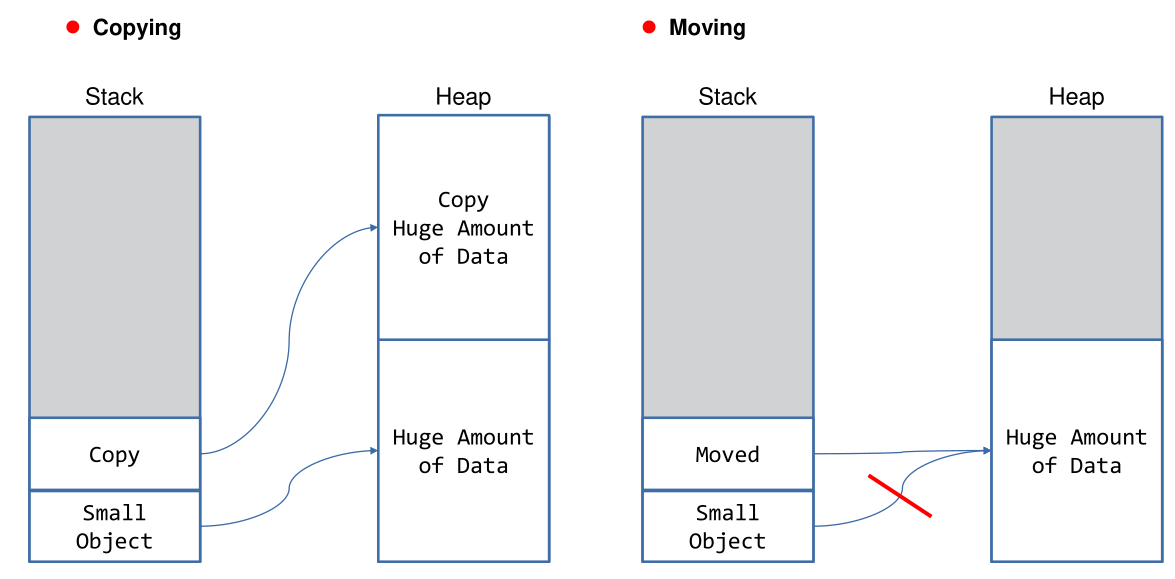
\includegraphics[width=.9\linewidth]{img/copy_vs_move_semantics.png}
\end{center}
\captionof{figure}{Copy vs move semantics}
}

\subparagraph{C++ References} \
\label{sec:org8a4b470}
In \href{../../../roam/20210920103243-c.org}{C++} references are not the same as in Java.
In \href{../../../roam/20210920103243-c.org}{C++} we have two kinds of references:
\begin{itemize}
\item \href{../../../roam/20230622083312-what_are_lvalue_references.org}{lvalue references}
\item \href{../../../roam/20230622083721-what_are_rvalue_references.org}{rvalue references}
\end{itemize}


\begin{itemize}
\item \texttt{void scale(Point point)}: No side-effect (call by value)
\item \texttt{void scale(Point \& point)}: Has side-effect (call by ref - lvalue reference)
\item \texttt{void scale(Point \&\& point)}: rvalue reference
\end{itemize}

\subparagraph{lvalue reference} \
\label{sec:org574c703}
lvalue references in C++ are just another name for a existing object.
The original must exists as long as it is referred to.
Do not return locales as reference)!
lvalue references binds to an \href{../../../roam/20230622085021-what_are_lvalues.org}{lvalue}.

The synatx for a lvalue reference is \texttt{T \&}.

\begin{lstlisting}[language=c++,label=lst:lvalue-reference-example,caption={lvalue reference example},captionpos=b,numbers=none]
auto modify(T& t) -> void {
  //manipulate t
}
auto lvalueRefExample() -> void {
  T t = 5;
  modify(t);
  T& ir = t;
  //...
}
\end{lstlisting}

\subparagraph{rvalue reference} \
\label{sec:org8fc8dd7}

rvalue references can extend the life-time of an temporary.
The synatx for an rvalue reference is \texttt{T \&\&}.
rvalue references binds to an rvalue (\href{../../../roam/20230622091114-what_are_xvalues.org}{xvalues}, \href{../../../roam/20230622085448-what_are_prvalues.org}{prvalues})


\begin{lstlisting}[language=c++,label=lst:rvalue-reference-example,caption={rvalue reference example},captionpos=b,numbers=none]
auto consume(Food&& food) -> void;
auto fryBurger() -> Food;
auto fastFood() -> void {
  Food fries{"salty and greasy"};
  consume(fryBurger());        //call with rvalue
  consume(fries);              //cannot pass lvalue to rvalue reference, does not compile
  consume(std::move(fries));   //explicit conversion lvalue to xvalue
  Food&& burger = fryBurger(); //life-extension of temporary
\end{lstlisting}

\subparagraph{Different value categories} \
\label{sec:org30a4834}
\begin{center}
\begin{tabular}{lll}
has identity? & can be moved from? & Value Category\\[0pt]
\hline
Yes & No & lvalue\\[0pt]
Yes & Yes & xvalue (expiring value)\\[0pt]
No & No (Since C++17) & prvalue (pure value)\\[0pt]
No & Yes (Since C++17) & - (does not exist anymore)\\[0pt]
\end{tabular}
\end{center}


{
\begin{center}
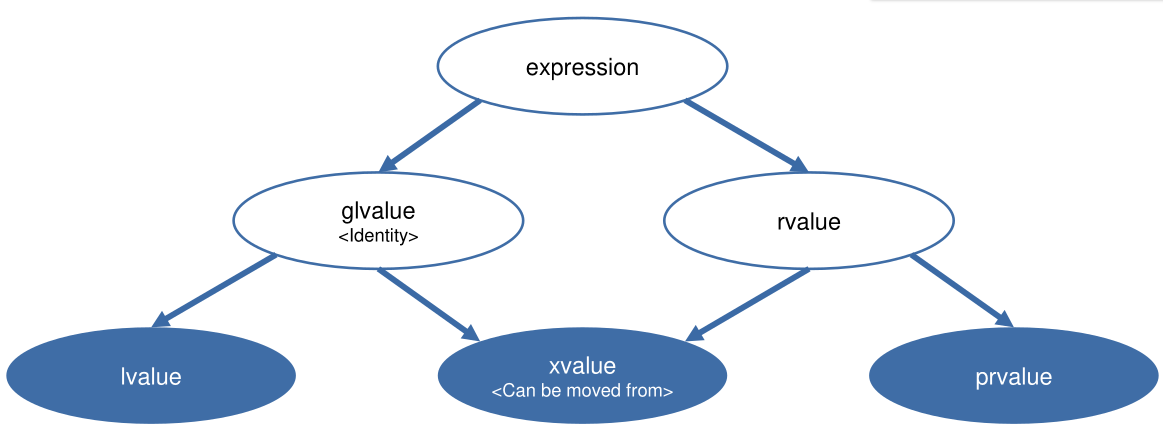
\includegraphics[width=.9\linewidth]{img/kinds_of_expressions.png}
\end{center}
\captionof{figure}{Kinds of expressions}\label{fig:kinds-of-expressions}
}

\subparagraph{lvalues} \
\label{sec:org88111f3}
Everything which belongs to the lvalue category can be bind by a lvalue reference.
\begin{itemize}
\item address can be taken
\item can be on the left-hand side of an assignment if modifiable (i.e. non-const)
\item can be used to initialize an lvalue reference
\end{itemize}


Examples for an lvalue:
\begin{itemize}
\item names of variables and parameters
\item function call with return type of lvalue reference to class type (\texttt{std::cout <{}<{} 23})
\item build-in prefix increment/decrement expressions (++a)
\item array index access (\texttt{arr[0]}), when \texttt{arr} is an lvalue
\item all string-literals by definition (\texttt{"name"})
\begin{itemize}
\item does not included user-defined literals like \texttt{"name"s} or \texttt{"name"sv}
\end{itemize}
\end{itemize}

\subparagraph{prvalues} \
\label{sec:org18c5f76}
\begin{itemize}
\item address can not be taken
\item can not be left-hand side argument of built-in assignment operators
\item temporary materialization when a gvalue is required
\begin{itemize}
\item conversion to xvalue
\end{itemize}
\end{itemize}


Examples for prvalues:
\begin{itemize}
\item literals: \texttt{23}, \texttt{false}, \texttt{nullptr}
\item function call expression of non-reference return type: \texttt{int std::abs(int n)}
\item serveral operators for built-in types, like post-increment / decremnt expressions: x++
\end{itemize}


temporary materialization (prvalue to xvalue) happens:
\begin{itemize}
\item when binding a reference to a prvalue (see 1 in \autoref{lst:example-for-conversion})
\item when accessing a member of a prvalue (see 2 in \autoref{lst:example-for-conversion})
\item when accessing an element of a prvalue array
\item when converting a prvalue array to a pointer
\item when initializing an \texttt{std::initializer\_list<T>} from a braced-init-list
\end{itemize}


\begin{lstlisting}[language=c++,label=lst:example-for-conversion,caption={Example for prvalue to xvalue conversion},captionpos=b,numbers=none]
struct Ghost {
  auto haunt() const -> void {
    std::cout << "booooo!\n";
  }
  //~Ghost() = delete;
};
auto evoke() -> Ghost {
  return Ghost{};
}
auto main() -> int {
  Ghost&& sam = evoke();  
  Ghost{}.haunt();
} 
\end{lstlisting}

\subparagraph{xvalues} \
\label{sec:orge1f4967}
\begin{itemize}
\item address can not be taken
\item can not be taken
\item can not be used as left-hand operator of built-in assignment
\item conversion from prvalue throught temporary materialization
\end{itemize}


Examples for an xvalue:
\begin{itemize}
\item function call with rvalue reference return type, like \texttt{std::move}: \texttt{std::move(x)}
\item access of non-reference members of an rvalue object
\item array index access (\texttt{arr[0]}), when \texttt{arr} is an rvalue
\end{itemize}


\begin{lstlisting}[language=c++,numbers=none]
X x1{}, x2{};
consume(std::move(x1));
std::move(x2).member;
X{}.member;
\end{lstlisting}


\subparagraph{Overload for references} \
\label{sec:org5007b84}
The overload for lvalue parameters impose ambiguities (you can not use lvalue and rvalue overloads).

{
\begin{center}
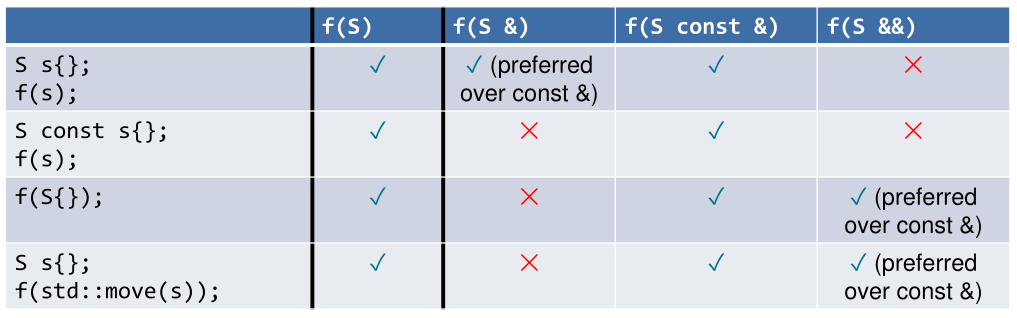
\includegraphics[width=.9\linewidth]{img/overloard_resolution_for_free_functions.png}
\end{center}
\captionof{figure}{Overloard resolution for free functions}\label{fig:overloard-resolution-for-free-functions}
}

{
\begin{center}
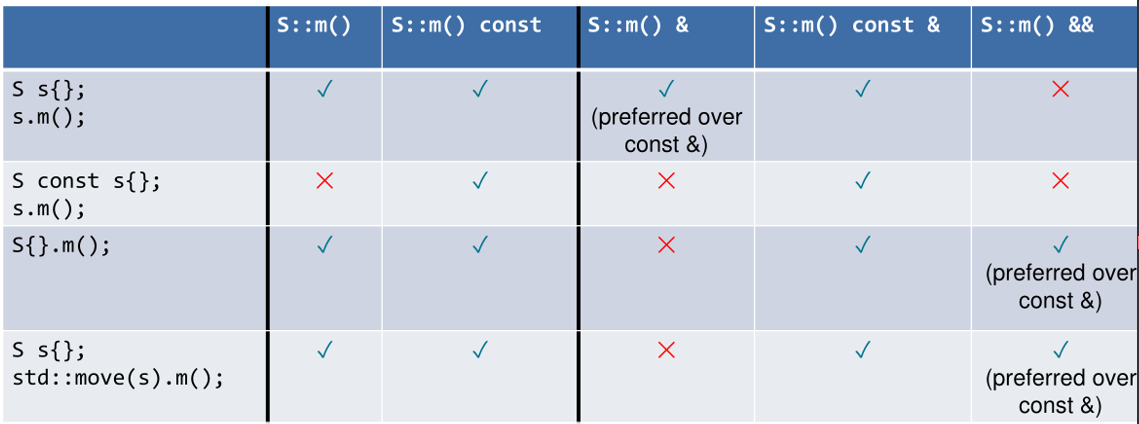
\includegraphics[width=.9\linewidth]{img/overload_resoulution_for_member_functions.png}
\end{center}
\captionof{figure}{Overloard resolution for member functions}\label{fig:overloard-resolution-for-member-functions}
}
\subparagraph{Move constructor} \
\label{sec:orge5abd84}
The move constructor is a type of constructors (\href{../../../roam/20211119152518-which_kind_of_constructor_exits_in_cpp.org}{Which kind of constructor exits in CPP?}) in \href{../../../roam/20210920103243-c.org}{CPP} to move all members to an new object.
\begin{lstlisting}[language=c++,numbers=none]
struct S {
  S(S && s) : member{std::move(s.member)}
  {}
  M member; 
};

auto f(S param) -> void {
  S local{std::move{param}}
}
\end{lstlisting}

\subparagraph{Copy constructor} \
\label{sec:orgb651fcd}
The copy constructor is a type of constructors (\href{../../../roam/20211119152518-which_kind_of_constructor_exits_in_cpp.org}{Which kind of constructor exits in CPP?}) in \href{../../../roam/20210920103243-c.org}{CPP} to copy all members to an new object.

\begin{lstlisting}[language=c++,numbers=none]
struct Date {
  Date(Date const &)
};
\end{lstlisting}

\subparagraph{Destructor} \
\label{sec:orge4708b4}
The Destructor is the counter part to the constructor (\href{../../../roam/20211119152518-which_kind_of_constructor_exits_in_cpp.org}{Which kind of constructor exits in CPP?}).
It must release all resources and is not allowed to throw an exception.
If you program properly you will hardly ever need to implement it yourself.
It is called automatically for local instances at the end of the block.
Must not rhow exceptions!

\begin{lstlisting}[language=c++,numbers=none]
class Date {
  ~Date();
};
\end{lstlisting}

\subparagraph{Copy assignment} \
\label{sec:orgc9d9dca}
If you need to implement the copy assignment operator you should follow the following points:
\begin{itemize}
\item avoid self-copy
\item use the copy constructor to create the copy of the argument
\item swap the \texttt{this} object with the copy (swapping is expected to be efficient)
\item Copy-Swap-Idiom
\end{itemize}


\begin{lstlisting}[language=c++,label=lst:example-for-copy-assignment,caption={Example for copy assignment},captionpos=b,numbers=none]
struct S {
  auto operator=(S const & s) -> S& {
    if (std::addressof(s) != this) {
      S copy = s;
      swap(copy)
        }
    return *this;
  }
};
\end{lstlisting}

\subparagraph{Move assignment} \
\label{sec:orgd6a3dec}
Usually you don't need to implment this at all.
If you have to, following the pattern is usually recommended:
\begin{itemize}
\item avoid self-move
\item swap the \texttt{this} object with the parameter
\end{itemize}


\begin{lstlisting}[language=c++,label=lst:example-for-a-move-assignment,caption={Example for a move assignment},captionpos=b,numbers=none]
struct S {
  auto operator=(S && s) -> S & {
    if (std::addressof(s) != this) {
      swap(s);
    }
    return *this;
  }
};
\end{lstlisting}

\subparagraph{What special members do you get?} \
\label{sec:orgfb1ca86}
{
\begin{center}
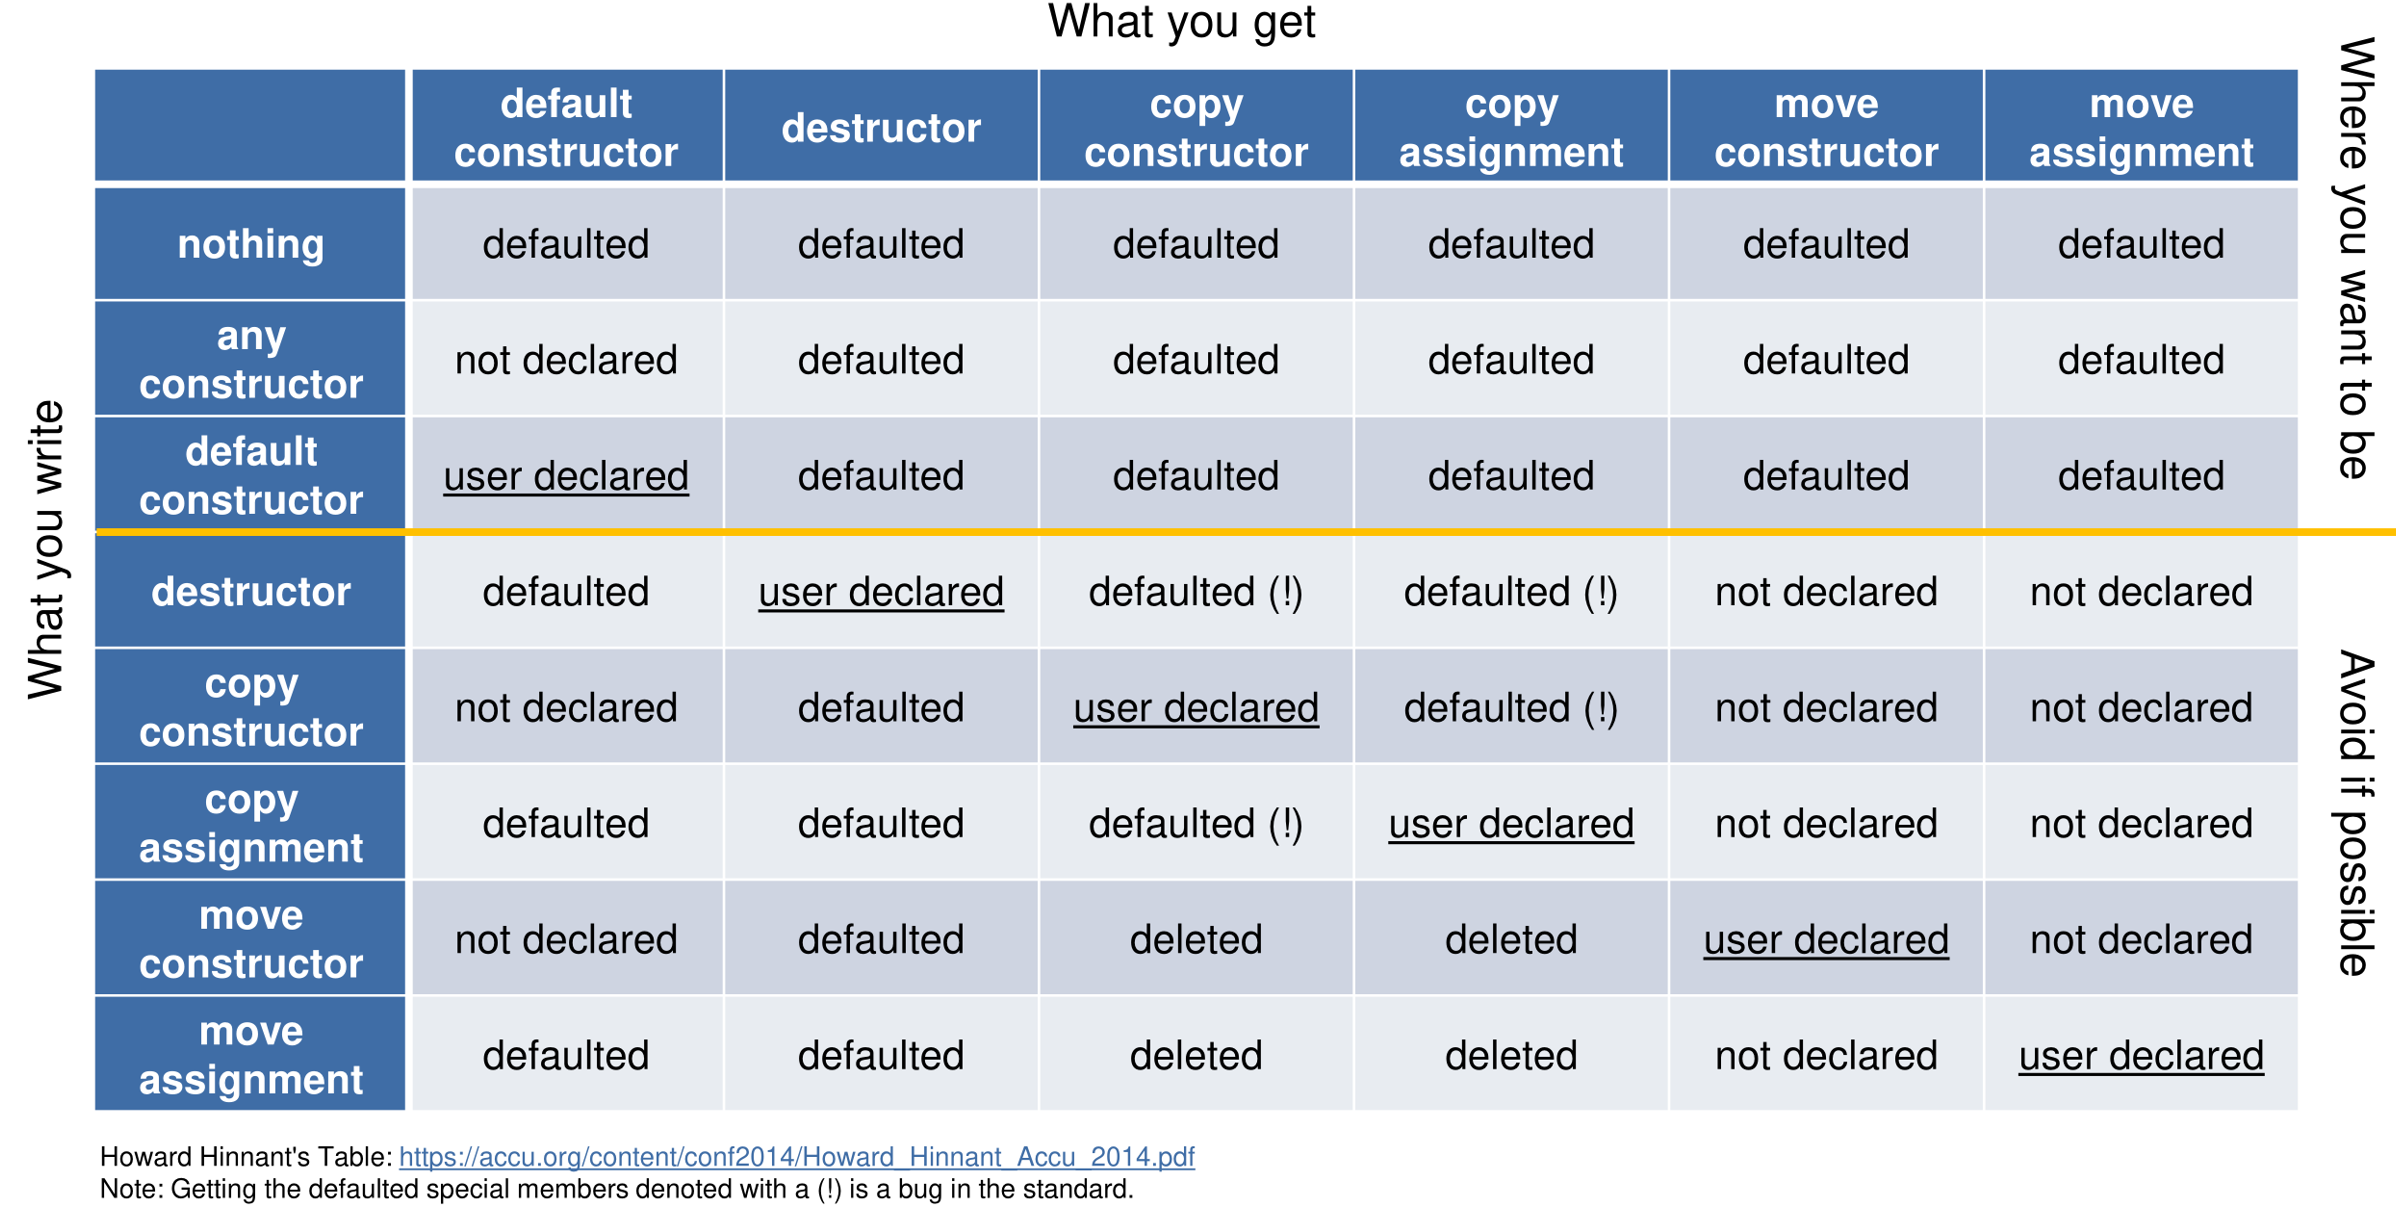
\includegraphics[width=.9\linewidth]{img/what_special_member_function_do_you_get.png}
\end{center}
\captionof{figure}{What special member function do you get?}\label{fig:what-special-member-function-do-you-get}
}
\subparagraph{Copy elision} \
\label{sec:org7e9766b}
In some cases the compiler is required to elide (omit) specific copy/move operations
Regardless of the side-effects of the corresponding special member functions!
\begin{itemize}
\item The omitted copy/move special member functions need not exist
\item If they exist, their side-effects are ignored
\end{itemize}


If initialization, when the initializer is a \href{../../../roam/20230622085448-what_are_prvalues.org}{prvalues} (see 1 in \autoref{lst:copy-elision-examples}) and when a function call returns a prvalue the compiler must omit the copy / move operations (see 2 in \autoref{lst:copy-elision-examples}).

\begin{lstlisting}[language=c++,label=lst:copy-elision-examples,caption={copy elision examples},captionpos=b,numbers=none]
auto create() -> S {
  return S{};
}
auto main() -> int {
  S s = S{S{}};             // 1
  S new_sw{create()};       // 2.1 
  S * sp = new S{create()}; // 2.2
}
\end{lstlisting}

The compiler is also allowed to optimize in throw and catch.
To be sure to avoid copies, catch by \texttt{const \&}.

\begin{lstlisting}[language=c++,label=lst:copy-elision-examples-try-catch,caption={copy elision examples try catch},captionpos=b,numbers=none]
try {
  throw S{7};
 } catch (...) {}


try {
  throw S{7};
 } catch (S s) {}
\end{lstlisting}

\subparagraph{Copy elision rules} \
\label{sec:orgcf5543f}
\begin{itemize}
\item NRVO (Named Return Value Optimization)
\begin{itemize}
\item return type is value type
\item return expression is a local variable (more or less) of the return type (const is ignored for type comparison)
\item the object is construced in the location of the return value (insted of moved or copied)
\end{itemize}
\item throw Expression
\begin{itemize}
\item return expression is a local variable from the innermost surround try block
\item the object is constructed in the location where it would be moved or copied
\end{itemize}
\item catch Clause
\begin{itemize}
\item if the caught type is the same as the object thrown, it access the object directly (as if caught by reference)
\end{itemize}
\end{itemize}

\section{Type Deduction}
\label{sec:orgfb132d7}
\subparagraph{Forwarding reference} \
\label{sec:orgee39c1b}
A forwarding reference can bind to an rvalue (\href{../../../roam/20230622085448-what_are_prvalues.org}{prvalues}, \href{../../../roam/20230622091114-what_are_xvalues.org}{xvalues}) and \href{../../../roam/20230622085021-what_are_lvalues.org}{lvalue}s depending on the context.
To create a forwarding reference, the function must be a template function.
If the function is part of a template class, the function must introduce a new template.


\begin{lstlisting}[language=c++,label=lst:example-for-forwarding-references,caption={Example for forwarding references},captionpos=b,numbers=none]
// template function
template <typename T>
auto f(T && param) -> void;

template <typename T>
struct S {
T member

// no forwarding reference
auto f(T && param) -> void {}
}

// forwarding reference
template <typename E>
auto g(E && param) -> void {}
}


int main() {
  int x = 23;
  f(x)  // lvalue

  f(23) // rvalue
}
\end{lstlisting}

\subparagraph{Type deduction} \
\label{sec:org686fdac}
\begin{lstlisting}[language=c++,label=fig:context,caption={Context},captionpos=b,numbers=none]
template <typename T>
auto f(ParamType param) -> void;
\end{lstlisting}

Deduction of type \texttt{T} depends on the structure of \texttt{ParamType}.
We have three cases:
\begin{enumerate}
\item \texttt{ParamType} is value type (\texttt{auto f(T param) -> void}) (\href{../../../roam/20230622105954-rules_for_type_deduction_with_value_type_in_cpp.org}{Rules for type deduction with value type in CPP})
\item \texttt{ParamType} is reference (\texttt{auto f(T \& param) -> void}) (\href{../../../roam/20230622110632-rules_for_type_deduction_with_reference_type.org}{Rules for type deduction with reference type in CPP})
\item \texttt{ParamType} is a forwarding reference (\texttt{auto f(T \&\& param) -> void}) (\href{../../../roam/20230622111511-rules_for_type_deduction_with_forwarding_reference_type.org}{Rules for type deduction with forwarding reference type})
\end{enumerate}


Type deduction with \texttt{std::initializer\_list} does not work.
\begin{lstlisting}[language=c++,label=lst:std_initializer_list-in-type-deduction,caption={std::initializer\textsubscript{list} in type deduction},captionpos=b,numbers=none]
template <typename T>
auto f(T param) -> void {}
f({23})  // error

template <typename T>
auto g(std::initializer_list<T> param) -> void {}
g({23})  // T = int, ParamType = std::initializer_list<int>
\end{lstlisting}

\subparagraph{Type deduction with value types} \
\label{sec:org31227b1}
\begin{lstlisting}[language=c++,label=fig:context-value,caption={Context},captionpos=b,numbers=none]
template <typename T>
auto f(T param) -> void;

f(<expr>);
\end{lstlisting}

Steps:
\begin{enumerate}
\item \texttt{<expr>} is a reference type: ignore the reference
\item ignore \texttt{const} of \texttt{<expr>} (outermost)
\item pattern match \texttt{<expr>}'s type against ParamType to figure out \texttt{T}
\end{enumerate}


{
\begin{center}
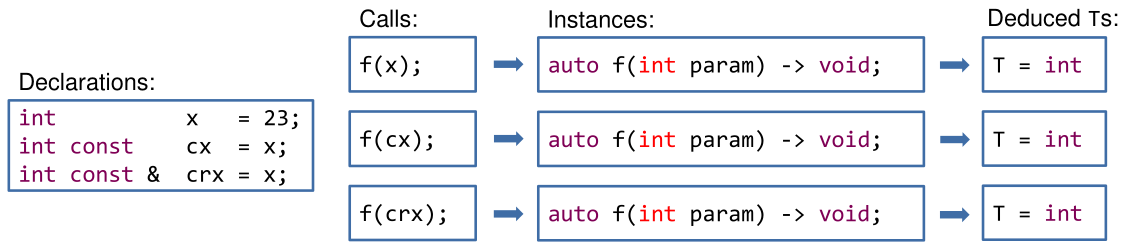
\includegraphics[width=.9\linewidth]{img/type_deduction_value_type.png}
\end{center}
\captionof{figure}{Example for type deduction with value type}\label{fig:example-for-type-deduction-with-value-type}
}

\subparagraph{Type deduction with reference types} \
\label{sec:org8366d9b}
\begin{lstlisting}[language=c++,label=fig:context-non-const,caption={Context non const},captionpos=b,numbers=none]
template <typename T>
auto f(T & param) -> void;

f(<expr>);
\end{lstlisting}

Steps:
\begin{enumerate}
\item \texttt{<expr>} is a reference type: ignore the reference
\item Pattern match \texttt{<expr>}'s type against ParamType to figure out T
\end{enumerate}


{
\begin{center}
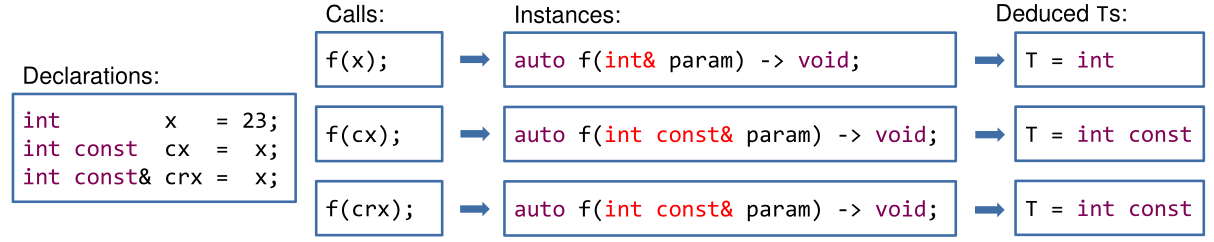
\includegraphics[width=.9\linewidth]{img/type_deduction_reference_type.png}
\end{center}
\captionof{figure}{Example for type deduction with reference type}\label{fig:example-for-type-deduction-with-reference-type}
}

\begin{lstlisting}[language=c++,label=fig:context-const,caption={Context const},captionpos=b,numbers=none]
template <typename T>
auto f(T const & param) -> void;

f(<expr>);
\end{lstlisting}

Steps:
\begin{enumerate}
\item \texttt{<expr>} is a reference type: ignore the reference
\item Pattern match \texttt{<expr>}'s type against ParamType to figure out T
\end{enumerate}


{
\begin{center}
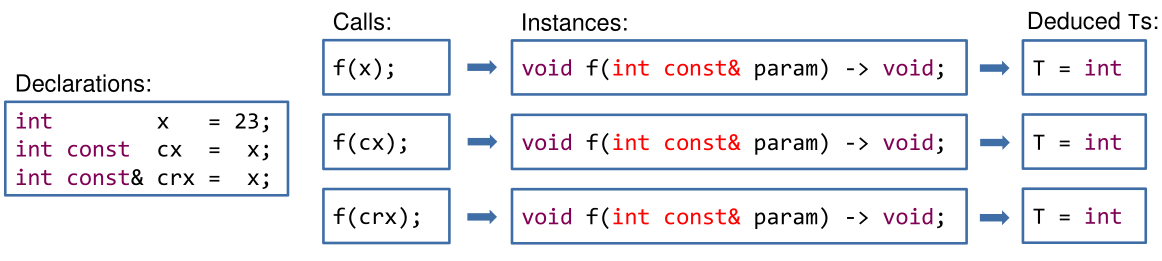
\includegraphics[width=.9\linewidth]{img/type_deduction_with_const_reference_type.png}
\end{center}
\captionof{figure}{Example for type deduction with const reference type}\label{fig:example-for-type-deduction-with-const-reference-type}
}
\subparagraph{Type deduction with forwarding reference types} \
\label{sec:orgd15ca0b}
\begin{lstlisting}[language=c++,label=fig:context-fwr,caption={Context},captionpos=b,numbers=none]
template <typename T>
auto f(T && param) -> void;

f(<expr>);
\end{lstlisting}

Steps:
\begin{enumerate}
\item \texttt{<expr>} is an lvalue: \texttt{T} and \texttt{ParamType} become lvalue references.
\item Otherwise (if \texttt{<expr>} is an rvalue): Rules for references apply (\href{../../../roam/20230622110632-rules_for_type_deduction_with_reference_type.org}{Rules for type deduction with reference type in CPP})
\end{enumerate}


{
\begin{center}
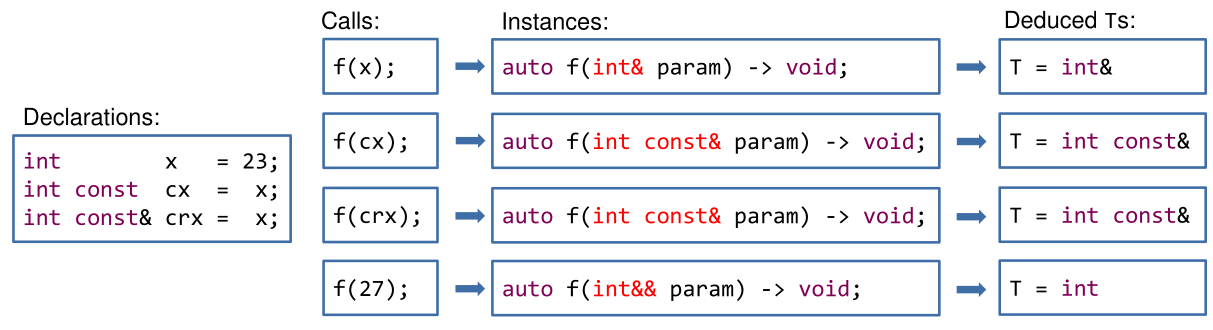
\includegraphics[width=.9\linewidth]{img/type_deduction_with_forwarding_references.png}
\end{center}
\captionof{figure}{Example for type deduction with forwarding reference type}\label{fig:example-for-type-deduction-with-forwarding-reference-type}
}
\subparagraph{Type deduction with auto} \
\label{sec:org057be65}
The type deduction with \texttt{auto} is the same as with templates (\href{../../../roam/20230622105606-rules_for_type_deduction_in_cpp.org}{Rules for type deduction in CPP}).
\texttt{auto} takes the place of \texttt{T}.

\begin{lstlisting}[language=c++,numbers=none]
auto x = 23;              //auto is a value type
auto const cx = x;        //auto is a value type
auto& rx = x;             //auto is a reference type

auto&& uref1 = x;         //x is an lvalue, uref1 is int&
auto&& uref2 = cx;        //cx is an lvalue, uref2 is int const&
auto&& uref3 = 23;        //23 is an rvalue, uref3 is int&&

auto init_list1 = {23};   //std::initializer_list<int>
auto init_list2{23};      //int, was std::initializer_list<int>1
auto init_list3{23, 23};  //Error, requires one single argument
\end{lstlisting}

\texttt{auto} can also be used as return type as well for parameter declarations in labmdas and functions.

\begin{lstlisting}[language=c++,label=lst:auto-as-function-parameter,caption={auto as function parameter},captionpos=b,numbers=none]
auto function(auto arg1, auto arg1) -> void {}

// results in this
template <typename T1, typename T2>
auto function(T1 arg1, T2 arg1) -> void {}

template <typename T>
concept Incrementable = requires (T const v){
  {v.increment()} -> std::same_as<T>;
};
auto increment(Incrementable auto value) -> T {
  return value.increment();
}
\end{lstlisting}

\subparagraph{Type deduction with decltype} \
\label{sec:org7b54017}
\texttt{decltype} can be applied to an expression: \texttt{decltype(x)}.
\texttt{decltype} represents the type of the applied expression.

\begin{lstlisting}[language=c++,label=lst:decltype-examples,caption={decltype examples},captionpos=b,numbers=none]
int            x       = 23;
int const      cx      = x;
decltype(cx)   cx_too  = cx; // type of cx_too is int const
int&           rx      = x;
decltype(rx)   rx_too  = rx; // type of rx_too is int&

auto           just_x  = rx; // type of just_x is int
decltype(auto) more_rx = rx; // type of more_rx is int&
\end{lstlisting}


\begin{lstlisting}[language=c++,numbers=none]
template <typename Container, typename Index>
decltype(auto) access(Container & c, Index i) {
  return c[i];
}

template <typename Container, typename Index>
auto access(Container & c, Index i) -> decltype(c[i]) {
  return c[i];
}
\end{lstlisting}

rules for \texttt{decltype(auto)}:
\begin{itemize}
\item unparenthesized variable name or data member: \texttt{T}, Type of the expression (retains reference)
\item expression of value category xvalue: \texttt{T\&\&}, rvalue reference
\item expression of value category lvalue: \texttt{T\&}, lvalue reference
\item expression of value category prvalue: \texttt{T}, value type of the expression
\end{itemize}


\begin{lstlisting}[language=c++,label=lst:example-for-decltype(auto),caption={Example for decltype(auto)},captionpos=b,numbers=none]
decltype(auto) funcName() {
  int local = 42;
  return local; //decltype(local) => int
}
decltype(auto) funcNameRef() {
  int local = 42;
  int & lref = local;
  return lref; //int & -> bad, dangling reference
}
decltype(auto) funcXvalue() {
  int local = 42;
  return std::move(local); //int && -> bad, dangling reference
}
decltype(auto) funcLvalue() {
  int local = 42;
  return (local); //int & -> bad, dangling reference
}
decltype(auto) funcPrvalue() {
  return 5; //int
}
\end{lstlisting}

\subparagraph{Perfect forwarding} \
\label{sec:org97dab5c}
\begin{lstlisting}[language=c++,label=lst:forwarding-reference-example,caption={Forwarding Reference example},captionpos=b,numbers=none]
template <typename T>
auto log_and_do(T&& param) -> void {
  //log
  do_something(std::move(param));
}
\end{lstlisting}

In \autoref{lst:forwarding-reference-example} param is a forwarding reference.
However, \texttt{param} is always an lvalue and \texttt{std::move(param)} always an rvalue.
If \texttt{T} is of reference type we want to pass an lvalue otherwise we want to pass an rvalue.
You can do this using \texttt{std::forward}.

\begin{lstlisting}[language=c++,label=lst:forwarding-reference-using-std-forward-example,caption={Forwarding Reference using std::forward example},captionpos=b,numbers=none]
template <typename T>
auto log_and_do(T&& param) -> void {
  //log
  do_something(std::forward(param));
}

Content c{};
log_and_do(c);
auto log_and_do(Content& param) -> void {
  do_something(std::forward<Content&>(param));
}

log_and_do(Content{});
auto log_and_do(Content&& param) -> void {
  do_something(std::forward<Content>(param));
}
\end{lstlisting}
\subparagraph{Inside std::forward} \
\label{sec:orge75a7bc}
The \texttt{std::forward} is used to forward an incoming reference to another function as the same type.
Therefore, \href{../../../roam/20230622083312-what_are_lvalue_references.org}{lvalue references} and \href{../../../roam/20230622083721-what_are_rvalue_references.org}{rvalue references} are forward as such.

\begin{itemize}
\item If \texttt{T} is of value type, a \texttt{T\&\&} is the result of the expression
\item If \texttt{T} is of lvalue reference type, a \texttt{T \& \&\&} is the result of the expression
\item If \texttt{T} is of rvalue reference type, a \texttt{T \&\& \&\&} is the result of the expression
\end{itemize}


A \texttt{T \& \&\&} is a rvalue reference to an lvalue reference, which collapse to a simple lvalue reference.
A \texttt{T \&\& \&\&} is a rvalue reference to an lvalue reference, which collapse to a simple rvale reference.

\begin{lstlisting}[language=c++,label=lst:std-forward-for-lvalue-references,caption={Example implementation for std::forward},captionpos=b,numbers=none]
template <typename T>
decltype(auto) forward(std::remove_reference_t<T> & param) {
  return static_cast<T&&>(param);
}

template <typename T>
decltype(auto) forward(std::remove_reference_t<T> && param) {
  return static_cast<T&&>(param);
}
\end{lstlisting}

\section{Heap Memory Management}
\label{sec:org0b69890}
\subparagraph{Pointers} \
\label{sec:orgc3c170f}
Pointer are things which point to a thing somewhere in the memory.


{
\begin{center}
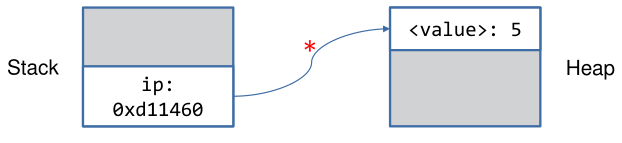
\includegraphics[width=.9\linewidth]{img/pointer_to_heap.png}
\end{center}
\captionof{figure}{Point from stack to heap}\label{fig:point-from-stack-to-heap}
}
To create an array on the heap you have to use the following synatx:
\begin{lstlisting}[language=c++,numbers=none]
auto arr = new int[5]{};
// or
int * arr2 = new int[5]{};
// arr and arr2 are pointesr to the first element
\end{lstlisting}

{
\begin{center}
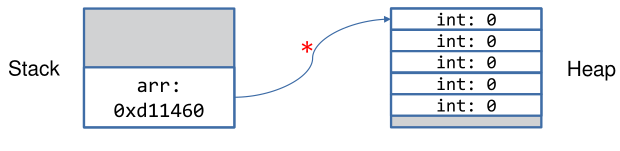
\includegraphics[width=.9\linewidth]{img/pointer_to_array.png}
\end{center}
\captionof{figure}{Pointer to array}\label{fig:pointer-to-array}
}

If you want to create a null pointer (a pointer which points nowhere), you should use \texttt{nullptr} instead of \texttt{0} or \texttt{NULL} (\texttt{NULL} is just an alias to \texttt{0}).

\begin{lstlisting}[language=c++,numbers=none]
auto bar(int i) -> void;
auto bar(S* ps) -> void;
//calls
bar(0);       //bar(int)
bar(NULL);    //surprising also bar(int)
bar(nullptr); //bar(S*)
\end{lstlisting}

\subparagraph{Allocate memory} \
\label{sec:org846e5f6}
To allocate new memory on heap, use the following syntax:
\begin{itemize}
\item \texttt{new <type> <initializer>}
\end{itemize}


However, you can not allocate an array of non-default constructible types.
However, you can allocate plain memory (\texttt{std::byte[]}) and initialize it later using \href{../../../roam/20230622180239-what_is_placement_new_in_cpp.org}{Placement new}.

\begin{lstlisting}[language=c++,label=lst:allocate-new-memory-on-heap,caption={Allocate new memory on heap},captionpos=b,numbers=none]
struct Point {
  Point(int x, int y) : x {x}, y {y}{}
  int x, y;
};

auto createPoint(int x, int y) -> Point* {
  return new Point{x, y}; //constructor
}

auto createCorners(int x, int y) -> Point* {
  return new Point[2]{{0, 0}, {x, y}};
}

auto defaultPoints(int x, int y) -> Point* {
  return new Point[2]{}; // does not work, because no default constructor
}
\end{lstlisting}

\begin{lstlisting}[language=c++,label=lst:example-for-a-non-default-constructible-type-on-the-heap,caption={Example for a non default constructible type on the heap},captionpos=b,numbers=none]
auto elementAt(std::byte * memory, size_t index) -> Point& {
  return reinterpret_cast<Point *>(memory)[index];
}
auto memory = std::make_unique<std::byte[]>(sizeof(Point) * 2); // allocate plain memory
Point * first = &elementAt(memory.get(), 0);
new (first) Point{1, 2};  // create new Point object in the alread allocated memory
Point * second = &elementAt(memory.get(), 1);
new (second) Point{4, 5};  // create new Point object in the alread allocated memory

std::destory_at(second);
std::destory_at(first);
\end{lstlisting}

\subparagraph{Deallocate memory} \
\label{sec:org41d2ea5}
To deallocate memory you have to distinguied between array and single objects:
\begin{itemize}
\item memory deallocation: \texttt{delete <pointer>}
\item array memory deallocation: \texttt{delete[] <pointer-to-array>}
\begin{itemize}
\item this deallocates also multidimensional arrays
\end{itemize}
\end{itemize}


Deleting a \texttt{nullptr} does nothing
However, deleting the same object twiche is \textbf{Undefined Behaviour}.
\subparagraph{Placement new} \
\label{sec:org9999eed}
If you already allocated some memory, you can construct an object to this location.
\begin{itemize}
\item \texttt{new (<location> <type> <initializer>})
\end{itemize}

This instruction does \textbf{NOT} allocate newy memory.

The same can also be done using the \texttt{std::construct\_at} from the std library.




\begin{lstlisting}[language=c++,numbers=none]
struct Point {
  Point(int x, int y) :
    x {x}, y {y}{}
  int x, y;
};
auto funWithPoint() -> void {
  auto ptr = new Point{9, 8};
  //must release Point{9, 8}
  new (ptr) Point{7, 6};
  delete ptr;
}
\end{lstlisting}

\subparagraph{Placement delete} \
\label{sec:org37c23b5}
If you want to destruct an object but you dont want to free the memory, you can call the destructor manually.
\begin{itemize}
\item \texttt{ptr->\textasciitilde{}S()}
\end{itemize}

This instruction does \textbf{NOT} free the memory

The same can also be done using the \texttt{std::destroy\_at} from the std library.


\begin{lstlisting}[language=c++,label=lst:example-for-placement-new-and-delete,caption={Example for placement new and delete},captionpos=b,numbers=none]
struct Resource {
  Resource() {
    /*allocate resource*/
  }
  ~Resource() {
    /*deallocate resource*/
  }
};
auto funWithPoint() -> void {
  auto ptr = new Resource{};
  std::destroy_at(ptr);
  // or ptr->~Resource();
  new (ptr) Resource{};
  delete ptr;
}
\end{lstlisting}

\subparagraph{Stack only class} \
\label{sec:org2384bc6}
If you want to prevent, that the user creates your data structure on the heap, you have to override the \texttt{new} and \texttt{delete} operators.
The \texttt{new} operator should throw an exception, while the \texttt{delete} operator does nothing.

\begin{lstlisting}[language=c++,label=lst:example-struct-with-overriden-operators,caption={Example struct with overriden operators},captionpos=b,numbers=none]
struct not_on_heap {
  static auto operator new(std::size_t sz) -> void * {
    throw std::bad_alloc{};
  }
  static auto operator new[](std::size_t sz) -> void * {
    throw std::bad_alloc{};
  }
  static auto operator delete(void *ptr) -> void noexcept {
    // do nothing, never called, but should come in pairs
  }
  static auto operator delete[](void *ptr) -> void noexcept {
    // do nothing, never called, but should come in pairs
  }
};
\end{lstlisting}

\section{Iterator und Tags}
\label{sec:orgbbd56b9}
\subparagraph{What is a type tag} \
\label{sec:org0fb6f50}
A tag type is a class, which is only used to mark capabilities of associated types.
Suach a tag type does not contain ayn members.
It is also possible to derive tag types from each other to "inherit" the capabilities.


\begin{lstlisting}[language=c++,numbers=none]
//Provides travelThroughSpace
struct SpaceDriveTag{};
//Provides travelThroughSpace and travelThroughHyperspace
struct HyperspaceDriveTag : SpaceDriveTag{};
//Provides travelThroughSpace and travelImprobably
struct InfniteProbabilityDriveTag : SpaceDriveTag{};
\end{lstlisting}

\subparagraph{Tags for dispatch} \
\label{sec:org7d48eb8}
You should implement traits!
You implement a trait using templates and set the tag.
For each concrete implementation you can now create a template specialization and set tag accordingly.
Then you create one public function (\texttt{travelTo}), which calls the dispachted functions with the tag (\texttt{travelToDispatch}).

\begin{lstlisting}[language=c++,label=lst:tag-for-dispatching-example,caption={Tag for dispatching example},captionpos=b,numbers=none]
struct SpaceDriveTag {};
struct HyperspaceDriveTag : SpaceDriveTag {};
struct InfiniteProbabilityDriveTag : SpaceDriveTag {};

struct MultiPurposeCrewVehicle;
struct GalaxyClassShip;
struct HeartOfGoldPrototype;

// Every Spaceship can travel through space
template <typename>
struct SpaceshipTraits {
  using Drive = SpaceDriveTag;
};

template <>
struct SpaceshiTraits<GalaxyClassShip> {
  using Drive = HyperspaceDriveTag;
};

template <typename Spaceshipt>
auto travelToDispatch(Galaxy destination, Spaceship& ship, SpaceDriveTag) -> void {
  ship.travelThroughSpace(destination);
}

template <typename Spaceshipt>
auto travelToDispatch(Galaxy destination, Spaceship& ship, InfiniteProbabilityDriveTag) -> void {
  while(destination != ship.travelImprobably());
}

template <typename Spaceship>
auto travelTo(Galaxy destination, Spaceship& ship) -> void {
  typename SpaceShipTraits<SpaceShip>::Drive drive{};
  travelToDispatch(destination, ship, drive);
}
\end{lstlisting}

\subparagraph{Iterator Tags} \
\label{sec:org53a6d49}
In CPP exits two kinds of iterators:
\begin{itemize}
\item input iterator
\item forward iterator
\item bidirectional iterator
\item random access iterator
\item output iterator
\end{itemize}


{
\begin{center}
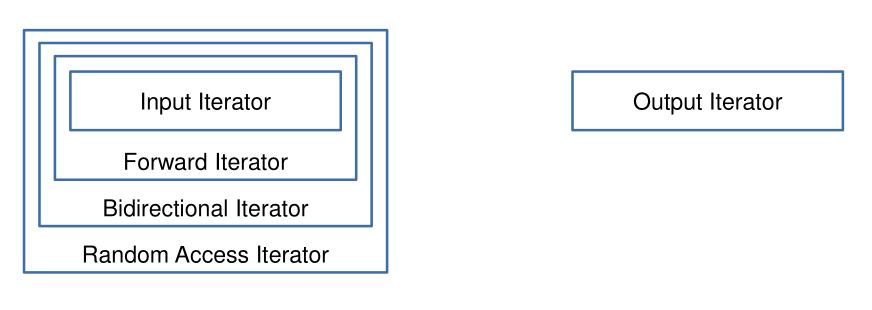
\includegraphics[width=.9\linewidth]{img/stl_iterator_categories.png}
\end{center}
\captionof{figure}{STL Iterator Categories}\label{fig:stl-iterator-categories}
}

\subparagraph{Iterator member types} \
\label{sec:orgf07d3b7}
\begin{table}[htbp]
\caption{\label{tbl:expected-members-in-a-cpp-iterator}Expected members in a C++ iterator}
\centering
\begin{tabular}{ll}
member & description\\[0pt]
\hline
iterator\_category & Specifies the iterator category by tag\\[0pt]
value\_type & Specifies the type of the elements the iterator iterates over\\[0pt]
difference\_type & Specifies the type used to specify iterator distance (ususally ptrdiff\textsubscript{t})\\[0pt]
pointer & Specifies the pointer type for the elements the iterator iterates over\\[0pt]
reference & Specifies the reference type for the elements the iterator iterates\\[0pt]
\end{tabular}
\end{table}


\begin{lstlisting}[language=c++,label=lst:example-member-types-for-an-iterator,caption={Example member types for an iterator},captionpos=b,numbers=none]
struct IntIterator {
  using iterator_category = std::input_iterator_tag;
  using value_type = int;
  using difference_type = ptrdiff_t;
  using pointer = int *;
  using reference = int &;
}
\end{lstlisting}

\subparagraph{Iterator\textsubscript{traits}<>} \
\label{sec:org7543e01}
\texttt{std::iterator\_traits} is used implement algorithms only based on this "interface".
Therefore, if a type provides all required properties, it can be used as an iterator.

\begin{lstlisting}[language=c++,label=lst:example-usage-of-iterator_traits,caption={Example usage of iterator\textsubscript{traits}},captionpos=b,numbers=none]
template <typename InputIter, typename Distance>
auto advanceImpl(InputIter & i, Distance d, std::input_iterator_tag) -> void {
  while (d--) { i++; }
}

template <typename RandomAccessIter, typename Distance>
auto advanceImpl(RandomAccessIter & i, Distance d, std::random_access_iterator_tag) -> void {
  i += d;
}

template <typename InputIter, typename Distance>
auto advance(Inputer & i, Distance n) -> void {
  typename std::iterator_traits<InputIter>::difference_type d = n;
  advanceImpl(i, d, std::iterator_traits<InputIter>::iterator_category{});
}
\end{lstlisting}

\subparagraph{Using Boost iterator} \
\label{sec:org358d51d}
\begin{lstlisting}[language=c++,numbers=none]
struct IntIteratorBoost
  : boost::input_iterator_helper<IntIteratorBoost, int> {
  explicit IntIteratorBoost(int start = 0)
    : value { start } {}
  auto operator==(IntIteratorBoost const& r) const -> bool {
    return value == r.value;
  }
  auto operator*() const -> value_type { return value; }
  auto operator ++() -> IntIteratorBoost& {
    ++value;
    return *this;
  }
private:
  value_type value;
};
\end{lstlisting}
\section{Advanced Templates}
\label{sec:org2621b01}
\subparagraph{Static polymorphism} \
\label{sec:org390601d}
Static polymorphism happens at compile-time and is therefore faster in the execution and the type checks happens at compile-time.
In C++ static polymorhism works using templates.
At compile time every call to the template, with an different type, is copied and the template parameter replaced with the type.

The drawback is, the compiler has to generate larger binary, the template code has to be known when used and the compile-time is longer.

\begin{lstlisting}[language=c++,label=lst:example-for-a-cpp-template,caption={Example for a C++ template},captionpos=b,numbers=none]
template <typename T>
auto f(T t) -> void {
  // do something
}

f(int);
// generates this
auto f(int t) -> void {
  // do something
}
\end{lstlisting}

\subparagraph{Dynamic polymorphism} \
\label{sec:org2f3b70d}
Dynamic polymorphism is when you have a inheritance hirarchy and you call a virtual function on the object.
This will then call the actual implementation on the object (not necessary the function on the base object).
The dynamic dispatch is performed using a \href{../../../roam/20221230181314-what_is_the_virtual_method_table.org}{vtable}.

\begin{lstlisting}[language=c++,numbers=none]
struct Shape {
  virtual unsigned area() const = 0;
  virtual ~Shape();
};
struct Square : Shape {
  Square(unsigned side_length)
    : side_length{side_length} {}
  unsigned area() const {
    return side_length * side_length;
  }
  unsigned side_length;
};

decltype(auto) amountOfSeeds(Shape const & shape) {
  auto area = shape.area(); // calls area function on Square
  return area * seedsPerSquareMeter;
};

amountOfSeeds(Square{1});
\end{lstlisting}


{
\begin{center}
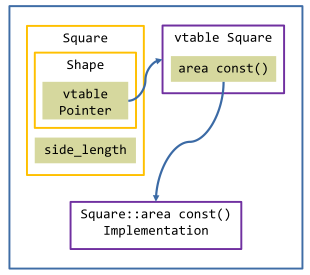
\includegraphics[width=.9\linewidth]{img/dynamic_dispatch.png}
\end{center}
\captionof{figure}{Dynamic Dispatch}\label{fig:dynamic-dispatch}
}
\subparagraph{SFINAE} \
\label{sec:org589fed6}
SFINAE stands for \emph{Substitution Failure Is Not An Error}.
When the C++ compiler performs overload resolution, the template parameters in a template declaration are substituted with the deducted types.
This can result in template instances that can not be compiled.
If the substituion of template parameters fails that overload candidate is discareded.

Substitution failure might happen in:
\begin{itemize}
\item function return type
\item function parameter
\item template parameter decleration
\item and expressions in the above
\end{itemize}


However, errors in the instance body are still errors.


{
\begin{center}
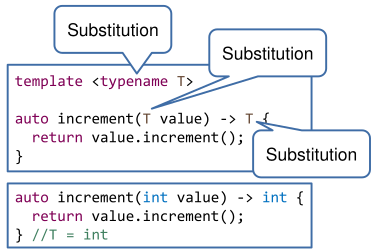
\includegraphics[width=.9\linewidth]{img/sfinae_locations.png}
\end{center}
\captionof{figure}{Positions for substituion}\label{fig:positions-for-substituion}
}
\subparagraph{How to use SFINAE?} \
\label{sec:org23adba7}
One solution might be to use \texttt{decltype} as trailing return type.
However, this does not always work (for example \texttt{void} as return type).
Instead you should use type traits from the \texttt{<type\_traits>} header.

\begin{lstlisting}[language=c++,label=lst:example-useage-for-sfinae,caption={Example useage for SFINAE},captionpos=b,numbers=none]
template <typename T>
auto increment1(T value) -> std::enable_if<std::is_class_v<T>, T> {
  return value.increment();
}

template <typename T>
auto increment2(std::enable_if_t<std::is_class_v<T>, T> value) -> T {
  return value.increment();
}

template <typename T, typename = std::enable_if_t<std::is_class_v<T>, void>>
auto increment3(T value) {
  return value.increment();
}

\end{lstlisting}

\subparagraph{Concepts} \
\label{sec:org3abfc4a}
Contraints are used to specify the characteristics of a type in template contextes.
\texttt{requires} clauses allow constraining template parameters.
\texttt{requires} is followed by a compile-time constatnt boolean expression.

\begin{lstlisting}[language=c++,label=lst:constraints-vs-sfinae,caption={constraints vs SFINAE},captionpos=b,numbers=none]
template <typename T>
requires std::is_class_v<T>
auto function1(T argument) -> void {}

template <typename T>
auto function2(T argument) -> void requires std::is_class_v<T> {}

template <typename T>
requires requires (T const v) { v.increment(); } // requires requires is not an error
auto increment(T value) -> T {
  return value.increment();
}

// SFINAE
template <typename T>
auto function3(T value) -> std::enable_if<std::is_class_v<T>, T> {}
\end{lstlisting}

\subparagraph{requires expressions} \
\label{sec:org07af21c}
The \texttt{requires} keyword can also be used to start an expression that evaluates to bool.
You can perform the following things:
\begin{itemize}
\item \textbf{simpel requirements} are statements that are true when they can be compiled
\item \textbf{type requirements} check wheter a specific tpye exists
\item \textbf{compound requirements} checks constraints on an expressions type
\item \textbf{nested requirements} contain further (nested) requires expression
\end{itemize}


\begin{lstlisting}[language=c++,label=lst:simple-requirements-examples,caption={simple requirements example},captionpos=b,numbers=none]
// simple requirements
template <typename T>
requires requires (T const v) { v.increment(); }
auto increment(T value) -> T {
  return value.increment();
}
\end{lstlisting}

\begin{lstlisting}[language=c++,label=lst:type-requirements-example,caption={type requirements example},captionpos=b,numbers=none]
// type requirements
template <typename T>
requires {
  typename BoundedBuffer<int>::value_type;
  typename BoundedBuffer<int>::size_type;
  typename BoundedBuffer<int>::reference;
  typename BoundedBuffer<int>::const_reference;
}
\end{lstlisting}

\begin{lstlisting}[language=c++,label=lst:compound-requirements-exmaple,caption={Compound requirements exmaple},captionpos=b,numbers=none]
// compound requirements
template <typename T>
requires requires (T const v) {
  { v.increment() } -> std::same_as<T>;
}
auto increment(T value) -> T {
  return value.increment();
}

template <typename T>
concept Incrementable = requires (T const v){
  {v.increment()} -> std::same_as<T>;
};
template <Incrementable T>
auto increment(T value) -> T {
  return value.increment();
}
template <typename T>
requires Incrementable<T>
auto increment(T value) -> T {
  return value.increment();
}
\end{lstlisting}

\subparagraph{Deduction guides} \
\label{sec:org7561fc2}
Deduction Guides are used to tell the compiler how to translate a set of constructor arguments into template parameters for the class.

In the following code snippet I have to tell the compiler how to map the Template Parameter \texttt{Iter}.
Otherwise, the compiler would not know that \texttt{Iter} should be an iterator.
It could be also an \texttt{int} or anything else.


\begin{lstlisting}[language=c++,numbers=none]
template <typename T>
class Sack {
  //...
  template <typename Iter>
  Sack(Iter begin, Iter end) : theSack(begin, end) {}
  //...
};

// deduction guide
template <typename Iter>
Sack(Iter begin, Iter end) -> Sack<typename std::iterator_traits<Iter>::value_type>;
\end{lstlisting}

\section{Compile Time Computation}
\label{sec:org184e135}
\subparagraph{constexpr contexts} \
\label{sec:orga42a225}
\begin{itemize}
\item non-type template arguments: \texttt{std::array<Element, 5> arr\{\};}
\item array bounds: \texttt{double matrix[ROWS][COLS]\{\};}
\item case expressions
\item enumerator initializers
\item static\textsubscript{assert}: \texttt{static\_assert(order =} 66)=
\item \texttt{constexpr} variables: \texttt{constexpr unsigned pi = 3;}
\item \texttt{constexpr if} statements: \texttt{if constexpr (size > 0)\{\}}
\item \texttt{noexcept}
\end{itemize}

\subparagraph{constexpr vs constinit} \
\label{sec:orgb770c52}
\texttt{consexpr} variables are \texttt{const} while \texttt{constinit} variables are non-const.
However, both are initialized at compile time.

\begin{lstlisting}[language=c++,label=lst:constexpr-and-constinit-initialization,caption={constexpr and constinit initialization},captionpos=b,numbers=none]
constexpr unsigned pi = 3;
constinit unsigned pi2 = 3;
\end{lstlisting}

\subparagraph{constexpr functions} \
\label{sec:orgd8a0b5a}
\texttt{constexpr} functions can be used to perform operations at compile-time.
A \texttt{constexpr} function can:
\begin{itemize}
\item have local variables of literal types
\item use loops, recursion, arrays, references
\item can contain branches with run-time features, if branch is not executed during compile-time computation
\item allocate dynamic memory (\texttt{new} / \texttt{delete}) that is cleandup by the end of the compilation
\item be a virtual member function
\item can only \texttt{constexpr} functions
\item can not use exception handling on executed path
\end{itemize}


\begin{lstlisting}[language=c++,label=lst:examples-for-constexpr-function-usage,caption={Examples for constexpr function usage},captionpos=b,numbers=none]
constexpr factorial(unsigned n) -> void {
  int local1;
  LiteralType local2{};
  std::string local3{};
}

consexpr auto allocate() -> int* {
  return new int{};
} //requires corresponding delete somewhere

struct Base {
  constexpr virtual auto modify() -> void;
};
\end{lstlisting}

\subparagraph{consteval functions} \
\label{sec:org852b539}
\texttt{consteval} functions are usable in \texttt{constexpr} contexts (see \href{../../../roam/20230629094857-what_are_constant_expression_contexts_in_cpp.org}{What are constant expression contexts in CPP?}) only.

\begin{lstlisting}[language=c++,label=lst:consteval-example,caption={consteval example},captionpos=b,numbers=none]
consteval auto factorial(unsigned n) {
  auto result = 1u;
  for (auto i = 2u; i <= n; i++) {
    result *= i;
  }
  return result;
}

constexpr auto factorialOf5 = factorial(5);

auto main() -> int {
  static_assert(factorialOf5 == 120);
  unsigned n;
  std::cin >> n;
  //std::cout << factorial(n); // does not compile
}
\end{lstlisting}

\subparagraph{UB in constexpr} \
\label{sec:orgf17a3ea}
The compiler will prevent Undefined Behaviour during constexpr evaluation and generates a compiler error.

\subparagraph{literal types} \
\label{sec:orgae5645b}
A literal type is one of the following:
\begin{itemize}
\item built-in scalar types (\texttt{int}, \texttt{double}, pointers, enumerations)
\item structs with some restrictions
\begin{itemize}
\item trivial destructor (non-user-defined)
\item with a \texttt{constexpr} / \texttt{constval} constructor
\end{itemize}
\item lambdas
\item references
\item arrays of literal types
\item void
\end{itemize}


Literal types can be usedin in \href{../../../roam/20230629095751-what_are_constexpr_functions_in_cpp.org}{constexpr function}s, but only \texttt{constexpr} member function can be called on values of literal types.

\subparagraph{literal class types} \
\label{sec:orga819e06}
To be a literal type the class must have:
\begin{itemize}
\item a trivial destructor (non-user defined)
\item at least one constexpr / constval constructor
\item constexpr / constval member functions (only those are usabel in constexpr context)
\end{itemize}


It is also possible to have non-constexpr constructors as well as non-constexpr member functions.

\begin{lstlisting}[language=c++,label=lst:example-for-a-literal-class-type,caption={Example for a literal class type},captionpos=b,numbers=none]
template <typename T>
class Vector {
  constexpr static size_t dimensions = 3;
  std::array<T, dimensions> values{};

public:
  constexpr Vector(T x, T y, T z)
    : values{x, y, z} {}

  constexpr auto length() const -> {
    auto squares = x() * x() +
        y() * y() +
        z() * z();
    return std::sqrt(squares);
  }

  constexpr auto x() -> T& {
    return values[0];
  }

  constexpr auto x() const -> T const & {
    return values[0];
  }
  // ...
}
\end{lstlisting}

\subparagraph{user-defined literals} \
\label{sec:org9dae6c2}
User-defined literals are a way to construct a class from a literal type.

\begin{lstlisting}[language=c++,label=lst:user-defined-literals-in-action,caption={User-defined literals in action},captionpos=b,numbers=none]
auto speed1 = Speed<Kph>{5.0};
auto speed2 = Speed<Mph>{5.0};
auto speed3 = Speed<Mps>{5.0};

// vs.

auto speed1 = 5.0_kph;
auto speed2 = 5.0_mph;
auto speed3 = 5.0_mps;
\end{lstlisting}

\subparagraph{create user-defined literals} \
\label{sec:orgb8423ac}
To create a user-defined literal you have to overwrite to operator for it.
The UDLSuffix could lexically be any identifier, but must start with an underscore.
Other suffixes are reserved for the standard.

Also put your UDL overloads that belong together in a sperate namespace and import them when required using \texttt{using namespace}.

\begin{lstlisting}[language=c++,label=lst:user-defined-literal-for-speed,caption={user-defined literal for Speed},captionpos=b,numbers=none]
namespace velocity::literals {
  constexpr inline auto operator"" _kph(unsigned long long value) -> Speed<Kph> {
    return Speed<Kph>{safeToDouble(value)};
  }

  constexpr inline auto operator"" _kph(long double value) -> Speed<Kph> {
    return Speed<Kph>{safeToDouble(value)};
  }
}

namespace mystring {
  inline auto operator"" _s(char const *s, std::size_t len) -> std::string {
    return std::string {s, len };
  }

  // works only for integral and floating literals
  // 42_ss becomes std::string{"42"}
  inline auto operator"" _ss(char const *s) -> std::string {
    return std::string { s }
  }
}
\end{lstlisting}

\section{Threading and Mutexes}
\label{sec:org31cd401}
\subparagraph{Threads} \
\label{sec:org42aacc6}
In CPP we have many different classes for threads:
\begin{itemize}
\item \texttt{std::thread}: is started automatically (\href{../../../roam/20230629112109-how_to_use_std_thread_in_cpp.org}{How to use std::thread in CPP?})
\item \texttt{std::jthread}: automatically calls \texttt{join}
\end{itemize}



\begin{lstlisting}[language=c++,label=lst:threads-in-cpp,caption={threads in CPP},captionpos=b,numbers=none]
auto main() -> int {
  std::thread greeter {
    []{ std::cout << "Hello, I'm thread!\n" }
  };
  greeter.join();
}
\end{lstlisting}

\subparagraph{std::thread} \
\label{sec:orge95fe9d}
A \texttt{std::thread} is started automatically after its creation.
To run a thread you have to provide a lambda, a function or a functor object which can be executed in a thread.
Return values are ignored.

If possible you should pass all arguments by value to avoid \href{../../../roam/20220323174221-what_is_a_data_race.org}{data race}s and danglign references.
If the thread goes out of scope you have to \texttt{join} or \texttt{detach} the thread.

\begin{lstlisting}[language=c++,caption={std::thread example},captionpos=b,numbers=none]
struct Functor {
  auto operator()() const -> void {
    std::cout << "Functor" << std::endl;
  }
};

struct function() -> void {
  std::cout << "Function" << std::endl;
}

auto main() -> int {
  std::thread functionThread{function};
  std::thread functorThread{Functor{}};
  std::thread lambdaThread{
    []{ std::cout << "Lambda" << std::endl; }
  };

  lambdaThread.join();
  functorThread.join();
  functionThread.join();
}
\end{lstlisting}

\subparagraph{Wake up a thread} \
\label{sec:org5226dad}
\begin{enumerate}
\item \texttt{notifyAll()}, \texttt{notify()}
\item InterruptedException (\href{../../../roam/20220228135733-the_interruptedexception_in_java.org}{The InterruptedException in Java})
\item Spurious Wake up (falsely wake up POSIX Thread API)
\end{enumerate}

\subparagraph{Mutexes} \
\label{sec:orgefd4c48}
In the C++ standard library we have four kinds of mutexes.
They can be devided into recursive and timed.

\begin{description}
\item[{recursive}] allow multiple nested acquire operations of the same thread (prevents self-deadlock)
\item[{timed}] also provides timed acquire operations (\texttt{try\_lock\_for / try\_lock\_until})
\end{description}


Each mutex has multiple operations defined (more for read-locking - \texttt{\_shared}):
\begin{itemize}
\item \texttt{lock()} - blocking
\item \texttt{try\_lock()} non-blocking
\item \texttt{unlock()} - non-blocking
\item \texttt{try\_lock\_for(<duration>)} - only for timed
\item \texttt{try\_lock\_until(<time>)} - only for timed
\end{itemize}


After each lock you must unlock the mutex, otherwise deadlocks can occurs.
To prevent this problem you can use RAII wrappers (\href{../../../roam/20230629135006-what_are_the_different_locks_for_mutexes.org}{What are the different locks for mutexes?}).


\begin{table}[htbp]
\caption{\label{tbl:various-mutexs-by-recursive-and-timed}Various mutexs by recursive and timed}
\centering
\begin{tabular}{|l|l|l|l|}
\hline
\multicolumn{2}{|l|}{} & \multicolumn{2}{l|}{Recursive} \\
\cline{3-4}
\multicolumn{2}{|l|}{} & No & Yes \\
\hline
Timed & No & std::mutex & std::recursive\_mute \\
\cline{2-4}
 & Yes & std::timed\_mutex & std::recursive\_timed\_mutex \\
\hline
\end{tabular}
\end{table}

\subparagraph{read-write locks} \
\label{sec:org9c9218e}
Mutual exclusion is too strong when only reading happens.
Mutual exclusion is only required when minimal one thread wants to write.

\begin{center}
\begin{tabular}{lll}
Parallel & Read & Write\\[0pt]
Read & Yes & No\\[0pt]
Write & No & No\\[0pt]
\end{tabular}
\end{center}


\begin{lstlisting}[language=java,numbers=none]
var rwLock = new ReentrantReadWriteLock(true);
rwLock.readLock().lock();
// read-only accesses
rwLock.readLock().unlock();
rwLock.writeLock().lock();
// write (and read) accesses
rwLock.writeLock().unlock();
\end{lstlisting}

\subparagraph{different locks} \
\label{sec:org2cda7dc}
Instead of locking and unlocking manually a mutex, you can use \href{../../../roam/20220118172628-resource_acquisition_is_initialization.org}{RAII} wrappers to automatically lock and unlock a mutex.

\begin{table}[htbp]
\caption{\label{tbl:raii-wrappers-for-mutexes}RAII wrappers for mutexes}
\centering
\begin{tabular}{|l|l|}
\hline
std::lock\_gurad & RAII wrapper for a single mutex \\
 & - Locks immediately when constructed \\
 & - Unlocks when destructed \\
\hline
std::scoped\_lock & RAII wrapper for multiple mutexes \\
 & - Locks immediately when constructed \\
 & - Unlocks when destructed \\
\hline
std::unique\_lock & Mutex wrapper that allows defered and timed locking \\
 & - Similar interface to timed mutex \\
 & - Allows explicit locking / unlocking \\
 & - Unlocks when destructed (if still locked) \\
\hline
std::shared\_lock & Wrapper for shared mutexes \\
 & - Allows explicit locking / unlocking \\
 & - Unlocks when destructed (if still locked) \\
\hline
\end{tabular}
\end{table}


\begin{lstlisting}[language=c++,label=lst:example-usage-for-raii-wrappers,caption={Example usage for RAII wrappers},captionpos=b,numbers=none]
template <typename T, tpyename MUTEX = std::mutex>
struct threadsafe_queue {
  using gurad std::lock_guard<MUTEX>;

  auto push(T const &t) -> void {
    guard lk{mx}; // acquire lock
    q.push(t);
  } // release lock

  auto empty() const -> bool {
    guard lk{mx};
    return q.empty();
  }

  auto swap(threadsafe_queue<T> & other) -> void {
    if (this == &other) return;

    std::scoped_lock both{mx, other.mx}; // lock multiple mutexes
    std::swap(q, other.q);
    // no need to swap mutex or condition variable
  }

private:
  mutable MUTEX mx{}; // must be mutable, otherwise you could not call empty
  std::queue<T> q{};
}
\end{lstlisting}

\subparagraph{lock and conditions} \
\label{sec:orgb894030}
In lock \& condition you have a monitor (\href{../../../roam/20220315074811-how_does_the_monitor_lock_work.org}{How does the monitor lock work?}), but instead of one queue you have a queue for each condition.
This has the benefit that not always all threads must be woken up.
Only the threads where the condition may be now fulfilled.


{
\begin{center}

\includegraphics[width=.9\linewidth]{img/lock_and_conditions.png}
\end{center}
\captionof{figure}{Lock \& Conditions}\label{fig:lock-and-conditions}
}
\subparagraph{std::condition\textsubscript{variable}} \
\label{sec:orgd4b4813}
\begin{lstlisting}[language=c++,label=lst:example-usage-std-condition_variable,caption={Example usage std::condition\textsubscript{variable}},captionpos=b,numbers=none]
template <typename T, typename MUTEX = std::mutex>
struct queue {
  using guard = std::lock_guard<MUTEX>;
  using lock = std::unique_lock<MUTEX>;

  auto push(T const & t) -> void {
    guard lk{mx};
    q.push(t);
    notEmpty.notify_one();
  }

  auto pop() -> T {
    lock lk{mx};
    notEmpty.wait(lk, [this] {
      return !q.empty();
    });
    T t = q.front();
    q.pop();
    return t;
  }

private:
  mutable MUTEX mx{};
  std::condition_variable notEmpty{};
  std::queue<T> q{};
};
\end{lstlisting}
\subparagraph{Return value from thread} \
\label{sec:orgb73f7a7}
In C++ we have \emph{futures} and \emph{promise} to communicate results from a thread to another.
The \texttt{std::future} represent results that may be computes asynchronously, while the \texttt{std::promise} is a possible origin for a future.

\begin{lstlisting}[language=c++,label=lst:example-usage-for-future-and-promise,caption={Example usage for future and promise},captionpos=b,numbers=none]
auto main() -> int {
  using namespace std::chrono_literals;

  std::promise<int> promise{};
  auto result = promise.get_future();

  auto thread = std::thread { [&]{
    std::this_thread::sleep_for(2s);
    promise.set_value(42); // communicate result
  }};

  std::this_thread::sleep_for(1s);

  std::cout << "The answer is: " << result.get() << '\n';
  thread.join();
}
\end{lstlisting}

\subparagraph{std::async} \
\label{sec:org84e8403}
Performing intesive computations on a different thread is a common task.
The C++ standard library uses for this the \texttt{std::async} class.
\texttt{std::async} returns a \texttt{std::future}.
Based on the \emph{launch policy} the execution is scheduled on the current thread (\texttt{std::launch:deferred}) or in a new thread (\texttt{std::launch::async}).
You should always the \emph{launch policy} because the standard does not define it uniquely. 

\begin{lstlisting}[language=c++,label=lst:example-usage-for-std-async,caption={Example usage for std::async},captionpos=b,numbers=none]
auto main() -> {
  auto the_answer = std::async(std::launch::async, [] {
    return 42;
  });

  std::cout << "The answer is: " << the_answer << '\n';
}
\end{lstlisting}

The \texttt{std::launch::async} policy performs the operation, regardless if the result is required.
Attention: the destructor will block until the result is availabel, but not in the \texttt{deferred} policy.
The \texttt{std::launch::deferred} policy performs the operation only if you need the result.
But the calculation is performed in the calling thread.

\section{Memory Model and Atomic}
\label{sec:org6c42d28}
\subparagraph{Memory Location} \
\label{sec:orgd381051}
In C++ a memory location must be one of the following types:
\begin{itemize}
\item arithmetic
\item pointer
\item enum
\item std::nullptr
\end{itemize}

\subparagraph{Memory Model} \
\label{sec:orgfc343a6}
Visibility of effects:
\begin{description}
\item[{sequenced-before}] withing a single thread
\item[{happens-before}] either sequenced-before or inter-thread happens-before
\item[{synchonizes-with}] inter-thread sync
\end{description}


Reads / Writes in a single statement are \textbf{unsequenced}!

For the memory ordering see \href{../../../roam/20230629160255-the_memory_ordering_in_cpp.org}{The memory ordering in CPP}.

\subparagraph{Memory Ordering} \
\label{sec:org094fbc2}
The memory orderings defi define when effects become visible:
\begin{description}
\item[{sequentially-consistent}] intuitive and the default behaviour
\item[{acquire / relase}] weaker guarantees than sequentailly-consistent
\item[{consume (do not use this)}] slightl weaker than acquire-release
\item[{relaxed}] no guarantees besides atomicity
\end{description}

\subparagraph{Atomics} \
\label{sec:org7374435}
In C++ atomics are realised using the \texttt{atomics} template.
atomics ar guaranteed to be data-race free.
\texttt{std::atomic\_flag} is guranteed to be lock-free.
All other atomics might use locks internally (for example for custom types).
However, they must be \textbf{trivially-copyable}.

All atomic operations take an additional argument to specify the memory ordering (\href{../../../roam/20230629160255-the_memory_ordering_in_cpp.org}{The memory ordering in CPP}):
\begin{itemize}
\item \texttt{std::memory\_order::seq\_cst}
\item \texttt{std::memory\_order::acquire}
\item \texttt{std::memory\_order::release}
\item \texttt{std::memory\_order::acq\_rel}
\item \texttt{std::memory\_order::release}
\end{itemize}


\begin{lstlisting}[language=c++,label=lst:example-for-atomic_flag,caption={Example for atomic\textsubscript{flag}},captionpos=b,numbers=none]
auto outputWhenReady(std::atomic_flag & flag, std::ostream & out) -> void {
  while (flag.test_and_set(std::memory_order::seq_cst)) yield();

  out << "Here is thread: "
        << get_id()
        << std::endl;
  flag.clear();
}
\end{lstlisting}

\subparagraph{Seq-Cst Ordering} \
\label{sec:orga199e32}
Using sequential consistency all operations are globally ordered.
Every thread will observe the same order.

The latest modification (in the global execution order) will be available to a read.

\subparagraph{Acquire / Release Ordering} \
\label{sec:org69b44ca}
Using the \emph{acquire} ordering no reads or writes in the current thread can be reordered \textbf{before} this load.
All writes in other threads that release \textbf{the same atomic} are visibile in the current thread.

\begin{lstlisting}[language=c++,numbers=none]
x.load(std::memory_order::acquire);
\end{lstlisting}

Using the \emph{release} ordering no reads or writes in the current thread can be reordered \textbf{after} this store.
All writes in the current thread are visible in other threads that acquire the same atomic.

\begin{lstlisting}[language=c++,numbers=none]
x.store(std::memory_order::release);
\end{lstlisting}

the \emph{acquire/release} works on the latest value.
\begin{lstlisting}[language=c++,numbers=none]
x.test_and_set(std::memory_order::acq_rel);
\end{lstlisting}

Note: It is not guaranteed that you always see the latest write in a read operation, but what you see is consistent according to the ordering above regarding the same atomic!

\subparagraph{Releaxed Ordering} \
\label{sec:org8ec7208}
The relaxed memory order does not give and guarantees about sequencing.
It guarantees only no data-races for atomic variables.

\begin{lstlisting}[language=c++,numbers=none]
x.store(true, std::memory_order::relaxed);
\end{lstlisting}

\subparagraph{Volatile} \
\label{sec:orgbeaf3dd}
The \texttt{volatile} keyword prevents the compiler from optimizing the varaible, even if the compiler can not see any visible side-effects within the same thread.
The compiler also does not reorder the instructions.
However, the hardware might still reorder instructions.

\begin{lstlisting}[language=c++,numbers=none]
volatile int mem{0};
\end{lstlisting}

\section{Networking}
\label{sec:org1b91071}
\subparagraph{Socket primites} \
\label{sec:orgbb4a34b}
\begin{table}[htbp]
\caption{\label{tbl:berkley-socket-primitives}Berkley socket primitives}
\centering
\begin{tabular}{ll}
Primitive & Meaning\\[0pt]
\hline
socket & create a new communication end point\\[0pt]
bind & attach a local address to a socket\\[0pt]
listen & announce willingness to accept connections\\[0pt]
accept & block caller until a connection request arrives\\[0pt]
connect & actively attempt to establish a connection\\[0pt]
send & send some data over the connection\\[0pt]
receive & receive some data over the connection\\[0pt]
close & release the connection\\[0pt]
shutdown & tear down the connection\\[0pt]
\end{tabular}
\end{table}

{
\begin{center}
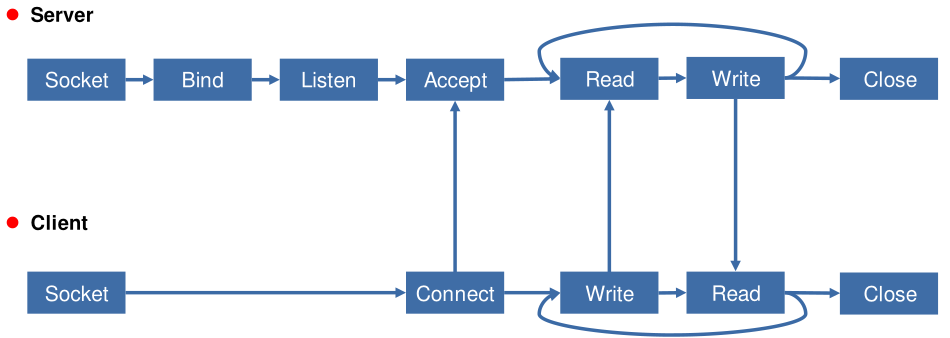
\includegraphics[width=.9\linewidth]{img/connection_oriented_communication_pattern.png}
\end{center}
\captionof{figure}{Connection-oriented communication pattern using sockets}\label{tbl:connection-oriented-communication-pattern-using-sockets}
}
\subparagraph{Sync TCP client} \
\label{sec:orgd2c10e1}
\begin{lstlisting}[language=c++,label=lst:client-connection-example-using-asio,caption={Client connection example using ASIO},captionpos=b,numbers=none]
auto main() -> int {
  asio::io_context context{};
  asio::ip::tcp::socket socket{context};
  auto address = asio::ip::make_address("127.0.0.1");
  auto endpoint = asio::ip::tcp::endpoint(address, 80);

  // asio::ip::tcp::resolver resolver{context};
  // auto endpoints = resolver.resolver(domain, "80"); // DNS
  socket.connect(endpoint);

  std::ostringstream request{};
  request << "GET / HTTP/1.1\r\n";
  request << "Host: " << domain << "\r\n";
  request << "\r\n";
  asio::write(socket, asio::buffer(request.str()));

  constexpr size_t bufferSize = 1024;
  std::array<char, bufferSize> reply{};
  asio::error_code errorCode{};
  auto readLength = asio::read(socket, asio::buffer(reply.data(), bufferSize), errorCode);

  socket.shutdown(asio::ip::tcp::socket::shutdown_both);
  socket.close();
}
\end{lstlisting}

\subparagraph{Sync TCP server} \
\label{sec:orgb34021d}
\begin{lstlisting}[language=c++,label=lst:server-example-using-asio,caption={Server example using ASIO},captionpos=b,numbers=none]
auto main() -> int {
  asio::io_context context{};
  asio::ip::tcp::endpoint localEndpoint{asio::ip::tcp::v4(), port};
  asio::ip::tcp::accptor acceptor{context, localEndpoint};

  asio::ip::tcp::endpoint peerEndpoint{};
  asio::ip::tcp::socket peerSocket = acceptor.accept(peerEndpoint);
}
\end{lstlisting}

\subparagraph{ASIO async operations} \
\label{sec:org05bd540}
\begin{enumerate}
\item the application invokes an async operation on an IO object and passes a completion handler as a callback
\item the IO object delegates the operation and the callback to its \texttt{io\_context}
\item the OS performs the async operation
\item the OS signals the \texttt{io\_context} that the operation has been completed
\item when the program calls \texttt{io\_context::run()} the remaining async operations are performed (wait for the result of the OS)
\item still inside \texttt{io\_context::run()} the completion handler is called to handle the result / error of the async operation
\end{enumerate}


{
\begin{center}
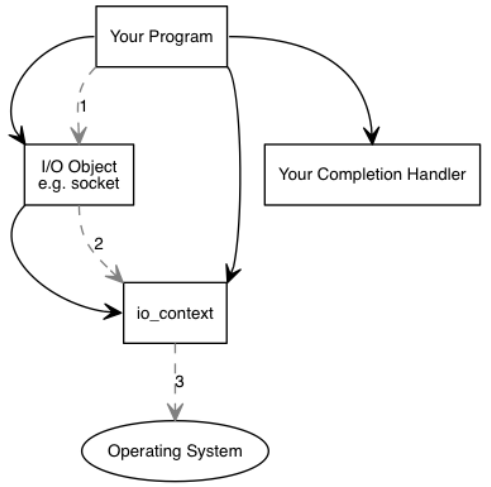
\includegraphics[width=.9\linewidth]{img/asio_async_operation.png}
\end{center}
\captionof{figure}{ASIO async operations part 1}\label{fig:asio-async-operations-part-1}
}

{
\begin{center}
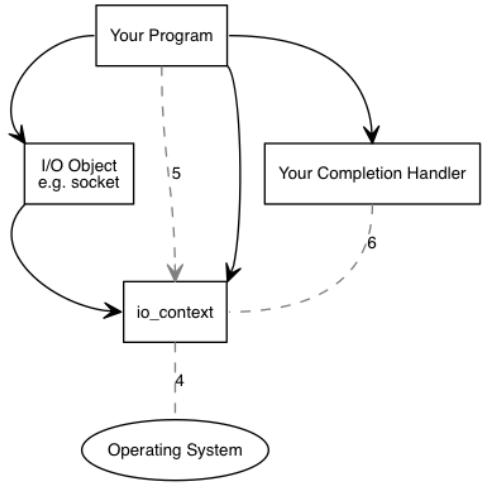
\includegraphics[width=.9\linewidth]{img/async_operations_2.png}
\end{center}
\captionof{figure}{ASIO async operations part 2}\label{fig:asio-async-operations-part-2}
}
\subparagraph{ASIO async example} \
\label{sec:org57a677d}
Make sure the \texttt{Server} lives as long as async operations on it are proccessed

\begin{lstlisting}[language=c++,label=lst:async-example-using-asio,caption={Async Example using ASIO},captionpos=b,numbers=none]
struct Session : std::enable_shared_from_this<Session> {
  explicit Session(asio::ip::tcp::socket socket);
  void start() {
        read;
  }

private:
  void read() {
        // using shared_from_this the session is kept alives
        auto handler = [self = shared_from_this()](error_code ec, size_t length) {}
  }
  void write(std::string data);

  asio::streambuf buffer{};
  std::istream input{&buffer};
  asio::ip::tcp::socket socket;
};

struct Server {
  using tcp = asio::ip::tcp;
  Server(asio::io_context & context, unsigned short port)
        : acceptor{context, tcp::endpoint{tcp::v4(), port}} {
        accept();
  }

private:
  void accept() {
        auto acceptHandler = [this](asio::error_code ec, tcp::socket peer) {
          if (!ec) {
            auto session = std::make_shared<Session>(std::move(peer));
            session->start(); //without the shared_from_this, the session would die here
          }
          accept();
        };
        acceptor.async_accept(acceptHandler);
  }

  tcp::acceptor acceptor;
};
\end{lstlisting}


{
\begin{center}
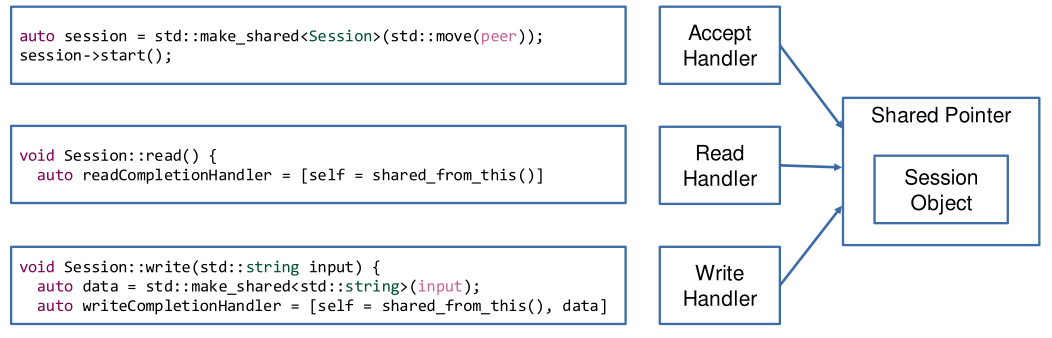
\includegraphics[width=.9\linewidth]{img/asio_keep_session_alive.png}
\end{center}
\captionof{figure}{Keep session alive}\label{fig:keep-session-alive}
}
\subparagraph{Signal handling} \
\label{sec:org8722f3c}
\begin{lstlisting}[language=c++,label=lst:example-for-signal-handling-using-asio,caption={Example for signal handling using ASIO},captionpos=b,numbers=none]
#include <asio.hpp>
#include <csignal>
#include <iostream>

auto main() -> int {
  auto context = asio::io_context{};

  auto signals = asio::signal_set{context, SIGINT, SIGTERM};
  signals.async_wait([&](auto error, auto sig) {
    if (!error) {
        std::cout << "received signal: " << sig << '\n';
    } else {
        std::cout << "signal handling aborted\n";
    }
  });

  context.run();
}
\end{lstlisting}

\section{Advanced Library Design}
\label{sec:org7b6980e}
\subparagraph{Exception Safety} \
\label{sec:org1790a0d}
In generic code (\href{../../../roam/20230629084234-cpp_template.org}{CPP Template}) you might call user-defined operations from the template argument.
The user-defined operations must not garble the data structure or leak resources.
At the same time, your template code is responsible that user-provided code does not suffer.

When an exception is thrown, "stack unwinding" destroys local and temporary objects.
If an exception is thrown during unwinding the program is terminated using \texttt{std::terminate()}.
To prevent this, you normally should not throw exceptions in the destructor.

To prevent all named problems you need to specify exception safty / exception guaranty.

\subparagraph{Exception Safety Levels} \
\label{sec:org627b767}
\begin{description}
\item[{noexcept / no-throw}] will never-ever throw an exception
\item[{strong exception safety}] operation succeeds and does not throw, or nothing happens but an exception is thrown (transaction)
\item[{basic exception safety}] does not leak resources or garble interanl data structures in case of an exception but might be incomplete
\item[{no guarantee}] undefined behaviour and garbled data lurking if exception is thrown (you dont want to go here)
\end{description}


A function can only be as exception-safe as the weakest sub-function it calls!


\begin{table}[htbp]
\caption{\label{tbl:overview-of-exception-safety-guarantees}Overview of Exception Safety Guarantees}
\centering
\begin{tabular}{llll}
 & Invariant OK & All or Nothing & Will not Throw\\[0pt]
No Guarantee & No & No & No\\[0pt]
Basic Guarantee & Yes & No & No\\[0pt]
Strong Guarantee & Yes & Yes & No\\[0pt]
No-Throw Guarantee & Yes & Yes & Yes\\[0pt]
\end{tabular}
\end{table}

\subparagraph{noexcept keyword} \
\label{sec:orgff2778f}
The \texttt{noexcept} keyword belongs to the function signature, but you can no overload on \texttt{noexcept}.
The compiler might optimize a call of a \texttt{noexcept} function better because it is not required to provide the infrastructure of uniwinding the stack.
However, if you throw in a \texttt{noexcept} environment the application terminates immediately.


\begin{lstlisting}[language=c++,label=lst:exaple-for-noexcept-in-signature,caption={Exaple for noexcept in signature},captionpos=b,numbers=none]
auto function() noexcept -> void {
  // ...
}

template <typename T>
auto function(T t) noexcept(true) -> void {
  // ...
}


template <typename T>
auto function(T t) noexcept(false) -> void {
  // ...
}
\end{lstlisting}

You can use the \texttt{noexcept} keyword also for conditions.

\begin{lstlisting}[language=c++,label=lst:example-for-conditional-noexcept,caption={Example for conditional noexcept},captionpos=b,numbers=none]
auto function2() noexcept(noexcept(function())) -> void {
  // function2 is noexcept when function() is also noexcept
}


auto main() -> int {
  std::cout << "is function() noexcept? " << noexcept(function()) << '\n';
}
\end{lstlisting}

\subparagraph{Throwing in member functions} \
\label{sec:org447e02a}
The destructor should normally not throw an exception.
During stack unwinding the destructor is called and if you then throw an exception the application terminates.

Move construction, move assignment and \texttt{swap} should not throw.
Copy can throw when new resources need to be allocated.

\subparagraph{wide vs narrow contracts} \
\label{sec:orgaf7e0a7}

A function that can handle all argument values of the given parameter types successfully has a "Wide Contract":
\begin{itemize}
\item it can not fail
\item it should be specified as \texttt{noexcept(true)}
\item \texttt{this} is also a parameter
\item globals and external resources also (e.g. heap)
\end{itemize}


A function that has preconditions on its parameters has a narrow contract:
\begin{itemize}
\item i.e., \texttt{int} parameter must not be zero
\item i.e., pointer parameter must not be \texttt{nullptr}
\item even if not checked and no excption thrown, those function should not be \texttt{noexcept}
\item this allows later checking and throwing if U.B.
\end{itemize}

\subparagraph{Standard Library Helpers} \
\label{sec:org117503f}
\begin{itemize}
\item \texttt{is\_nothrow\_constructible}
\item \texttt{is\_nothrow\_default\_constructible}
\item \texttt{is\_nothrow\_copy\_constructible}
\item \texttt{is\_nothrow\_move\_constructible}
\item \texttt{is\_nothrow\_assignable}
\item \texttt{is\_nothrow\_copy\_assignable}
\item \texttt{is\_nothrow\_move\_assignable}
\item \texttt{is\_nothrow\_destructible}
\item \texttt{is\_nothrow\_swappable}
\end{itemize}
\subparagraph{Opaque Types} \
\label{sec:org04ccf2d}

For an opaque type we do not know anything about its structure but its name.
This is achived using a forward declaration.

\begin{lstlisting}[language=c++,label=lst:example-for-an-opaque-type,numbers=none]
struct S; // Forward declaration
auto foo(S & s) -> void {
  foo(s);
  //S s{}; // Invalid
}

struct S{}; // Definition
auto main() -> int {
  S s{};
  foo(s);
}
\end{lstlisting}

\subparagraph{PIMPL Idiom} \
\label{sec:org018cc46}
If you make changes to a class definition, the client must be recompiled.
Even then, when the changes are not visible from outside.
Using PIMPL this can be neglected.

In the \emph{exported} header file you write a class consisting of a \textbf{Pointer to Implementaiton} and all public members of the real implementation.

\begin{lstlisting}[language=c++,caption={PIMPL example using shared\textsubscript{ptr}},captionpos=b,numbers=none]
// Wizard.hpp
class Wizard {
  // class WizardImpl is a forward declaration
  std::shared_ptr<class WizardImpl> pImpl;

public:
  Wizard(std::string name = "Rincewind");
  auto domagic(std::string wish) -> std::string;
};

// WizardImpl.cpp
class WizardImpl {
  std::string name;
  /// ...
public:
  WizardImpl(std::string name = "Rincewind") :
    name{name} {}
  auto doMagic(std::string const & wish) -> std::string {}
};

Wizard::Wizard(std::string name) :
  pImpl{std::make_shard<WizardImpl>(name)} {}

auto Wizard::doMagic(std::string wish) -> std::string {
  return pImpl->doMagic(wish);
}
\end{lstlisting}

\subparagraph{PIMPL with unique\textsubscript{ptr}} \
\label{sec:org7231674}
If you want to implement the PIMPL idiom using an \texttt{unique\_ptr} you must define the desturcotr (\href{../../../roam/20211119155746-the_destructor_in_cpp.org}{The Destructor in CPP}) manually in the class declaration.
This is required, because the default delter for the \texttt{unique\_ptr} has to know, how big the implementation is.
Therefore, you have to implement the destructor \textbf{after} the implementation again with \texttt{default}.

\begin{lstlisting}[language=c++,label=lst:pimpl-using-unique_ptr,caption={PIMPL using unique\textsubscript{ptr}},captionpos=b,numbers=none]
// Wizard.hpp
class Wizard {
  std::unique_ptr<class WizardImpl> pImpl;
public:
  Wizard(std::string name);
  ~Wizard();
  auto doMagic(std::string wish) -> std::string;
};

// WizardImpl.cpp
class WizardImpl {
  // ...
};


// Default the destructor
Wizard::~Wizard() = default;
\end{lstlisting}

\subparagraph{PIMPL and Copy} \
\label{sec:org020e109}
\begin{center}
\begin{tabular}{|l|l|}
\hline
No copying - only & std::unique\_ptr$<$class Impl$>$ \\
moving & - declare destructor \& = default \\
 & - declare move operations \& = default \\
 & \\
\hline
Shallow copying & std::shared\_ptr$<$class Impl$>$ \\
(Sharing the & \\
implementation) & \\
\hline
Deep copying & std::unique\_ptr$<$class Impl$>$ \\
(default for C++) & - with DIY copy constructor (use copy \\
 & constructor of Impl) \\
\hline
\end{tabular}
\end{center}

\section{Hour Glass Interface}
\label{sec:orgceb7ada}
\subparagraph{Hour Glass Interface} \
\label{sec:orgec13a35}
An hourglass interface is a way to expose your C++ library over a C ABI to another language (or C++).


{
\begin{center}
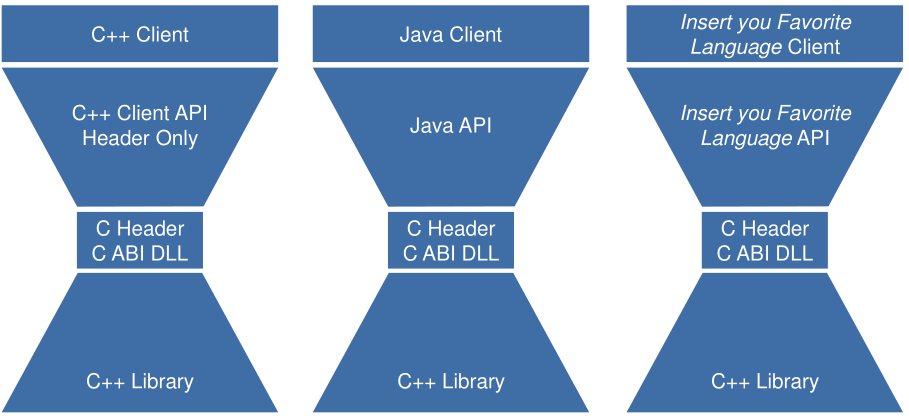
\includegraphics[width=.9\linewidth]{img/hourglass_interface.png}
\end{center}
\captionof{figure}{Hourglass Interface idea}\label{fig:hourglass-interface-idea}
}
\subparagraph{C++ to C ABI} \
\label{sec:org8561bc0}
Abstract data types can represented by pointers (\texttt{void *}).
Member functions map to functions taking the abstract data type pointer as first argument.
Constructors and destructors are replaced with factory and disposal functions.
Strings can only represented by \texttt{char *}.
Exception do not work across the C ABI.

\subparagraph{C++ in extern C} \
\label{sec:orgc900ea4}
C++ has a lot more features than C has.
Therefore, you can not use all features in an \texttt{extern "C"} interface:

\begin{itemize}
\item functions, but no template or variadic
\item C primitive types (\texttt{char}, \texttt{int}, \texttt{double}, \texttt{void})
\item pointers, including function pointers
\item forward-declared structs
\begin{itemize}
\item pointers to those are opaque types
\item are used for abstract data types
\end{itemize}
\item enums (unscoped - wouthout class or base type)
\end{itemize}


\begin{lstlisting}[language=c++,label=lst:example-for-a-extern-c-interface,caption={Example for a extern C interface},captionpos=b,numbers=none]
#ifdef __cplusplus
extern "C" {
#endif

  typedef struct Wizard * wizard;
  typedef struct Wizard const * cwizard;
  wizard createWizard(char const * name, error_t * out_error);
  void disposeWizard(wizard toDispose);

#ifdef __cplusplus
}
#endif
\end{lstlisting}

\subparagraph{Full C++ using extern C} \
\label{sec:orgccae2ac}
In the \texttt{extern C} interface we can only use a subset of C++ (\href{../../../roam/20230706185259-what_parts_of_cpp_can_be_used_in_an_extern_c_interface.org}{What parts of CPP can be used in an extern C interface?}).
So that we can use full C++ we have to create a so-called trampolin class.

\begin{lstlisting}[language=c++,label=lst:example-for-a-trampolin-class,caption={Example for a trampolin class},captionpos=b,numbers=none]
// Wizard.cpp
extern "C" {
  struct Wizard { // C linkage trampolin
    Wizard(char const * name)
    : wiz{nmae} {}

    unseen::Wizard wiz;
  };
}

// WizardHidden.hpp
namespace unseen {
  struct Wizard {
    // ...
    Wizard(std::string name = "Rincewind")
    : name{name}, wand{} {}

    auto doMagic(std::string const & wish) -> char const *;
    auto getName() const -> char const * {
        return name.c_str();
    }
  };
}
\end{lstlisting}

\subparagraph{Exception in extern C} \
\label{sec:org74dbaec}
In \texttt{extern C} we can not use exception and we must use pointers to pointers.
If an error occurs (exception) we have to allocate error value on the heap and provide a disposal function to clean up error.
To convert an exception to an error, we just capture everything and create an error when required.
We use a pointer to a pointer as referenec to a pointer.
Therefore, \texttt{out\_error} must not be \texttt{nullptr};

On the client side we can use \href{../../../roam/20220118172628-resource_acquisition_is_initialization.org}{RAII} wrappers to convert errors again into exceptions.


\begin{lstlisting}[language=c++,numbers=none]
// Wizard.cpp
extern "C" {
  template<typename Fn>
  bool translateExceptions(error_t * out_error, Fn && fn)
    try {
        fn();
        return true;
    } catch (const std::exception & e) {
        *out_error = new Error{e.what()};
        return false;
    } catch (...) {
        *out_error = new Error{"Unkown internal error"};
        return false;
    }

  wizard create_wizard(const char * name, error_t * out_error) {
    wizard result = nullptr;
    translateException(out_error, [&] {
        result = new Wizard{name};
    });
    return result;
  }
}
\end{lstlisting}

\section{Build Automation}
\label{sec:orga79d9f5}
\subparagraph{Build Automation Software} \
\label{sec:org91a2f04}
You can seperate into two classes of build automation software:
\begin{itemize}
\item Make-style build tools
\begin{itemize}
\item run build scripts
\item produce your final products
\end{itemize}
\item Build Script Generators
\begin{itemize}
\item generate configuration for make-style build systems
\item configuration independent of actual build tool
\item advanced features (download dependencies, \ldots{})
\end{itemize}
\end{itemize}


\subparagraph{cmake} \
\label{sec:org7a2739e}
When the flag is \texttt{PUBLIC}, a libraries or executables which links against it will inherit the properties.
Therefore, libraries should be \texttt{PUBLIC} and executables \texttt{PRIVATE} because you cannot link against an executable.


\begin{lstlisting}[language=sh,label=lst:example-for-cmakelists-txt,caption={Example for CMakeLists.txt},captionpos=b,numbers=none]
cmake_minimum_required(VERSION "3.12.0")

project("my_lib" LANGUAGES CXX)

add_library("my_lib" "lib.cpp")
target_include_directories("my_lib" PUBLIC "includes")
target_compile_features("my_lib" PUBLIC "cxx_std_17")
set_target_properties("my_lib" PROPERTIES
                      CXX_STARNDARD_REQUIRED YES
                      CXX_EXTENSIONS NO)


add_executable("my_app" "app.cpp")
target_link_libraries("my_app" PRIVATE "my_lib")
\end{lstlisting}

\begin{lstlisting}[language=sh,label=lst:build-cmake-project,caption={Build cmake project},captionpos=b,numbers=none]
mkdir build
cd build
cmake ..
cmake --build .
\end{lstlisting}

\subparagraph{Project Layout} \
\label{sec:org90a480f}
{
\begin{center}
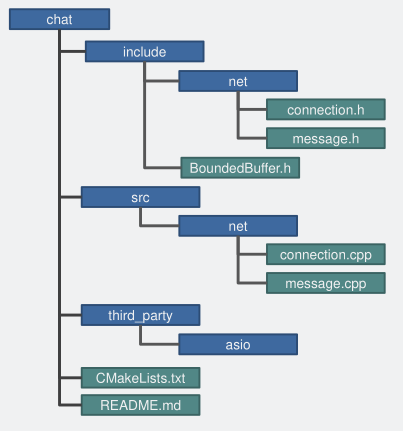
\includegraphics[width=.9\linewidth]{img/cpp_project_layout_app.png}
\end{center}
\captionof{figure}{Recomended project layout for an application}\label{fig:recomended-project-layout-for-an-application}
}


{
\begin{center}
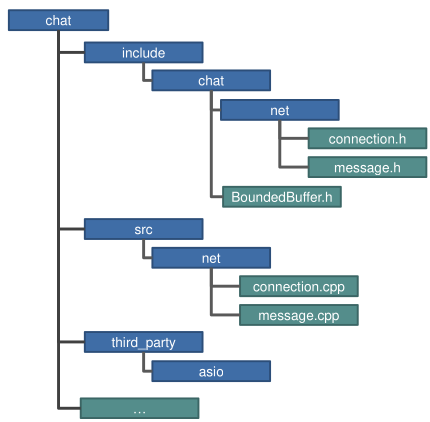
\includegraphics[width=.9\linewidth]{img/cpp_project_layout_library.png}
\end{center}
\captionof{figure}{Recomended project layout for a library}\label{fig:recomended-project-layout-for-a-library}
}

\end{multicols}
\end{document}